% Tipe dokumen adalah report dengan satu kolom kertas A4 satu sisi.
% Ukuran font 12pt
\documentclass[12pt, a4paper, onecolumn, twoside, final]{report}

% Load konfigurasi LaTeX untuk tipe laporan thesis
\usepackage{ta}
\usepackage{longtable}
\usepackage{booktabs}
\usepackage{siunitx}
\usepackage[indonesian]{babel}
\addto\captionsindonesian{
  \def\refname{Daftar Pustaka}% 
  \def\contentsname{Daftar Isi}%
}

% --- TAMBAHAN UNTUK PENGATURAN NOMOR HALAMAN --- %
% \usepackage{fancyhdr}
% \usepackage{etoolbox}
% \pagestyle{fancy}
% \fancyhf{}

% \fancyhead[RO]{\thepage}  % Halaman ganjil - kanan atas
% \fancyhead[LE]{\thepage}  % Halaman genap - kiri atas

% \fancypagestyle{chapterstart}{
%   \fancyhf{}
%   \fancyfoot[C]{\thepage}  % Nomor halaman di bawah tengah
% }

% \let\oldchapter\chapter
% \renewcommand{\chapter}{%
%   \clearpage
%   \cleardoublepage
%   \thispagestyle{chapterstart}
%   \oldchapter
% }
% --- TAMBAHAN SELESAI --- %

% --- TAMBAHAN UNTUK PENGATURAN NOMOR HALAMAN --- %
\usepackage{fancyhdr}
\usepackage{etoolbox}

% 1. Definisikan style untuk bagian ROMAWI (semua nomor di KANAN ATAS)
\fancypagestyle{romanstyle}{%
  \fancyhf{}% Kosongkan semua header/footer
  \fancyfoot[C]{\thepage}% Nomor halaman di Tengah Bawah (Center)
  \renewcommand{\headrulewidth}{0pt}%
  \renewcommand{\footrulewidth}{0pt}%
}

% 1. Definisikan style untuk halaman utama (pojok atas)
\fancypagestyle{mainstyle}{%
  \fancyhf{}%
  \fancyhead[RO]{\thepage}% Halaman ganjil - kanan atas
  \fancyhead[LE]{\thepage}% Halaman genap - kiri atas
  \renewcommand{\headrulewidth}{0pt}% Menghilangkan garis header
}

% 2. Definisikan style untuk halaman awal bab (tengah bawah)
\fancypagestyle{chapterstart}{%
  \fancyhf{}%
  \fancyfoot[C]{\thepage}%
}

% 3. Atur agar setiap \chapter menggunakan style 'chapterstart'
\let\oldchapter\chapter
\renewcommand{\chapter}{%
  \if@openright\cleardoublepage\else\clearpage\fi
  \thispagestyle{chapterstart}%
  \oldchapter
}
% --- TAMBAHAN SELESAI --- %


% Load konfigurasi khusus untuk laporan yang sedang dibuat
%-----------------------------------------------------------------------------%
% Informasi Mengenai Dokumen
%-----------------------------------------------------------------------------%
% 
% Judul laporan. 
\var{\judul}{Tes}
% 
% Tulis kembali judulnya, kali ini akan diubah menjadi huruf kapital
\Var{\Judul}{JUDUL}
% 
% Tulis kembali judul laporan namun dengan bahasa Inggris
\Var{\JudulInggris}{JUDUL BAHASA INGGRIS}
\Var{\JudulIndo}{JUDUL BAHASA INDONESIA}

% SESUAIKAN YAH! TUGAS AKHIR ATAU PROPOSAL 
% Tipe laporan, dapat berisi Skripsi, Tugas Akhir, Thesis, atau Disertasi 
\var{\type}{Skripsi}
% 
% Tulis kembali tipe laporan, kali ini akan diubah menjadi huruf kapital
\Var{\Type}{SKRIPSI}
% 
% Tulis nama penulis 
\var{\penulis}{Nama Penulis}
\var{\alamat}{Alamat Penulis}
\var{\tlp}{xxx}
\var{\email}{xxx@binus.ac.id}
% 
% Tulis kembali nama penulis, kali ini akan diubah menjadi huruf kapital
\Var{\Penulis}{NAMA PENULIS}
% 
% Tulis NPM penulis
\var{\nim}{XXXXXXX}
% 
% Tuliskan Fakultas dimana penulis berada
\Var{\Fakultas}{School of Computer Science}
\var{\fakultas}{School of Computer Science}
% 
% Tuliskan Program Studi yang diambil penulis
\Var{\Program}{Computer Science Study Program}
\var{\program}{Computer Science Study Program}
% 
% Tuliskan tahun publikasi laporan
\Var{\Tahun}{2025}
% 
% Tuliskan gelar yang akan diperoleh dengan menyerahkan laporan ini
\var{\gelar}{Sarjana Teknik}
% 
% Tuliskan tanggal pengesahan laporan, waktu dimana laporan diserahkan ke 
% penguji/sekretariat
\var{\tanggalPengesahan}{\today} 
% 
% 
% Tuliskan pembimbing 
\var{\pembimbingSatu}{Rissa Rahmania, S.T., M.T.}
\var{\nikSatu}{D6408}
\var{\pembimbingDua}{Prof. Dr. Ir. Derwin Suhartono, S.Kom., MTI}
\var{\nikDua}{0}
% 
% Alias untuk memudahkan alur penulisan paa saat menulis laporan
\var{\penulisSatu}{Mahasiswa 1}
\var{\NIMpenulisSatu}{0000000001}
\var{\penulisDua}{Mahasiswa 2}
\var{\NIMpenulisDua}{0000000002}
\var{\penulisTiga}{Mahasiswa 3}
\var{\NIMpenulisTiga}{0000000003}

%-----------------------------------------------------------------------------%
% Judul Setiap Bab
%-----------------------------------------------------------------------------%
% 
% Berikut ada judul-judul setiap bab. 
% Silahkan diubah sesuai dengan kebutuhan. 
% 
\var{\abstrak}{Abstrak}
\Var{\kataPengantar}{Kata Pengantar}
\Var{\babSatu}{Pendahuluan}
\Var{\babDua}{Tinjauan Pustaka}
\Var{\babTiga}{Metode Penelitian}
\Var{\babEmpat}{Hasil dan Pembahasan}
\Var{\babLima}{Simpulan dan Saran}


% Awal bagian penulisan laporan
\begin{document}

% Sampul Laporan

\begin{titlepage}
    \begin{center}      
        % judul thesis harus dalam 14pt Times New Roman
        \bo{\large{\JudulIndo}} \\[0.75cm]

        % \bo{\large{\JudulInggris}} \\ [0.75cm]

        \vspace*{0.7 cm}
        \bo{\large{\Type}}  \\
        \vspace*{0.7 cm} 
        
        % \textit{\bo{\JudulInggris}} \\[1.0cm]

        \vspace*{0.1 cm}    
        % harus dalam 14pt Times New Roman
        %\bo{\Type}
        
        % penulis dan npm
        \bo{oleh}\\
        % \vspace*{0.25 cm}
        \bo{\large{\Penulis}} \\
        % \vspace*{0.25 cm}
        \bo{\large{\nim}} \\     

        \vspace*{0.7 cm}
        
        \begin{figure}
            \begin{center}
                
\includegraphics[width=0.7\linewidth]{pic/logo.png}
            \end{center}
        \end{figure}
        
        % informasi mengenai fakultas dan program studi
       
        \bo{\doublespacing
                \large{\program}\\
                \large{\fakultas} \\
        	\large{Universitas Bina Nusantara}\\
        	\large{BANDUNG} \\
        	\large{2025}
        }
    \end{center}
\end{titlepage}


%comment dari sini%

\pagenumbering{gobble}

% Halaman pengesahan
% \addChapter{LEMBAR PENGESAHAN}
% % \chapter*{}
% \addcontentsline{toc}{section}{Pengesahan}
\thispagestyle{plain}
% 
% \vspace*{-3cm}
% \noindent Halaman Persetujuan Dosen Pembimbing 
\begin{center}      
        % \bo{Pernyataan Kesiapan Skripsi Untuk Ujian Pendadaran}
        % judul thesis harus dalam 14pt Times New Roman
        \bo{{\JudulIndo}} \\[0.75cm]

        % \bo{{\JudulInggris}} \\ [0.75cm]
        \bo{SKRIPSI}
        
        % \textit{\bo{\JudulInggris}} \\[1.0cm]

        \vspace*{0.1 cm}    
        % harus dalam 14pt Times New Roman
        %\bo{\Type}
        
        % penulis dan npm
        \bo{Disusun oleh}\\
        % \vspace*{0.25 cm}
        % \bo{{\penulis}} \\
        % \vspace*{0.25 cm}
        % \bo{{\nim}} \\ 
        \vspace{3cm}
       \begin{tabular}{>{\centering\arraybackslash}p{4cm}>{\centering\arraybackslash}p{4cm}>{\centering\arraybackslash}p{4cm}}

        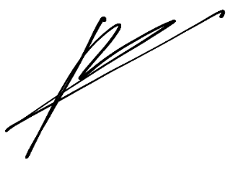
\includegraphics[height=1.8cm, width=3.5cm, keepaspectratio]{pic/rizkiafdl_signature.png} &
        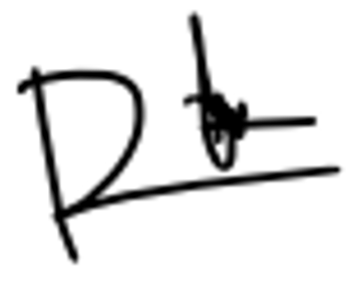
\includegraphics[height=1.8cm, width=3.5cm, keepaspectratio]{pic/rakha_picture.png} &
        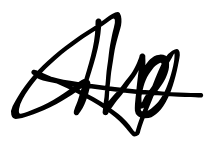
\includegraphics[height=1.8cm, width=3.5cm, keepaspectratio]{pic/ttdtheo.png} \\[4pt]

        \underline{\makebox[3.8cm][c]{\penulisSatu}} & \underline{\makebox[3.8cm][c]{\penulisDua}} & \underline{\makebox[3.8cm][c]{\penulisTiga}} \\[4pt]

        \fontsize{12}{14}\selectfont\bf{\NIMpenulisSatu} & \fontsize{12}{14}\selectfont\bf{\NIMpenulisDua} & \fontsize{12}{14}\selectfont\bf{\NIMpenulisTiga} \\

        \end{tabular}

        \vspace*{0.7 cm}
        % \bo{{\Type}}  \\
        % \vspace*{0.7 cm}

        \bo{Disetujui oleh}:\\
        \bo{Pembimbing dan Head of Study Program}\\
\end{center}

    % \vspace{\baselineskip}
    \vspace{1.5cm}
        
    \begin{center}
    \begin{minipage}{12cm}
        \centering
        % \hrulefill\\
        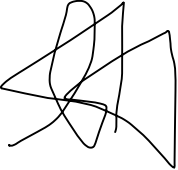
\includegraphics[height=1.8cm, width=5.5cm, keepaspectratio]{pic/pak_budi_signature.png}\\[4pt]
        \underline{\pembimbingSatu} \\[4pt]
        \fontsize{12}{14}\selectfont\bf{\nikSatu}\\
    \end{minipage}
    \end{center}

    % \vspace{1.5cm}
    % \renewcommand{\arraystretch}{0.7} 
    % \begin{center}
    %     \begingroup
    %     \begin{tabular}{ccc}
    %     % \hrulefill & & \hrulefill \\
    %     \underline{\pembimbingDua} & & \underline{\pembimbingTiga} \\
    %     \fontsize{12}{0}\bf{KO-PROMOTOR 1} & & \fontsize{12}{0}\bf{KO-PROMOTOR 2}\\
    %     \end{tabular}
    % \end{center}

    % \begin{center}\setstretch{2.0}{Mengetahui,}\end{center}

    \vspace{2cm}
    % \begin{center}
    %     \begin{minipage}{10cm}
    %     \centering
    %     % \hrulefill\\
    %     % \underline{\pembimbingDua}  \\[4pt]
    %     % \fontsize{12}{14}\selectfont\bf{Head of Computer Science Study Program}\\
    %     \end{minipage}
    % \end{center}

 
  
    

%comment disini%

% Gunakan penomoran halaman romawi
\pagenumbering{roman}
\pagestyle{romanstyle}
% setelah bagian ini, halaman dihitung sebagai halaman ke 2
\setcounter{page}{2}

%comment sini%

% Sampul ke dua
% \chapter*{}
% \cleardoublepage
% \newpage
% \phantomsection
% \pagenumbering{roman}
\thispagestyle{plain}
    \begin{center}      
        % judul thesis harus dalam 14pt Times New Roman
        \bo{\large{\JudulIndo}} \\[0.75cm]

        \vspace*{0.7 cm}
        \bo{\large{\Type}}  \\
        % \vspace*{0.7 cm} 
        
        \vspace*{0.1 cm}    
        % \bo{
            \textbf{diajukan sebagai salah satu syarat} \\
            \textbf{untuk gelar kesarjanaan pada} \\
            \textbf{Program Studi Teknik Informatika} \\
            \textbf{Jenjang Pendidikan Strata-1} \\ 
        % }
        \vspace*{0.5cm}
        
        % penulis dan npm
        \bo{oleh}\\
        % \vspace*{0.25 cm}
        \bo{\large{\penulis}} \\
        % \vspace*{0.25 cm}
        \bo{\large{\nim}} \\     



        \begin{figure}
            \centering
            
\includegraphics[width=0.5\linewidth]{pic/logo.png}
        \end{figure}
       
        \bo{\doublespacing
                \large{\program}\\
                \large{\fakultas} \\
        	\large{Universitas Bina Nusantara}\\
        	\large{BANDUNG} \\
        	\large{2025}
        }
    \end{center}
% \end{titlepage}


% Halaman pernyataan orisinalitas
% \addChapter{LEMBAR PERNYATAAN ORISINALITAS}
% \chapter*{}
\thispagestyle{plain}
    % \vspace*{-3cm}
    % \noindent Halaman Pernyataan Orisinalitas 
    \begin{center}
    \textbf{Universitas Bina Nusantara}\\
    \vspace*{-0.5cm}
    \rule{13cm}{1pt} \\
    \vspace*{-0.2cm}
    \textbf{Pernyataan Kesiapan Skripsi untuk Ujian Pendadaran}
    \end{center}

% \AddToShipoutPicture*{%
% \gradientbox{white}{white}{%

% \begin{minipage}[ct][0.98\paperheight][t]{\paperwidth}%
%         \begin{figure}
%         		\hspace{1 cm}
%         		\vspace{1 cm}
% \centering
%             \begin{center}
%                 \includegraphics[scale=0.74]{pics/orisinalitas.png}
%             \end{center}
%         \end{figure}
% \end{minipage}}}

    % \vspace*{1 cm}
    \textbf{Pernyataan Penyusunan Skripsi}\\
    \indent\textbf{Kami}, 

    % \begin{itemize}
    %     \item \textbf{\penulisSatu}
    %     \item \textbf{\penulisDua}
    %     \item \textbf{\penulisTiga}
    % \end{itemize}
    \indent\textbf{\penulisSatu} \\
    \indent\textbf{\penulisDua} \\
    \indent\textbf{\penulisTiga},

    \textbf{dengan ini menyatakan bahwa Skripsi yang berjudul}: 

    \begin{center}
    \textbf{\Judul}\\
    \textit{\textbf{\JudulInggris}}\\
    \end{center}
    
    % \vspace*{1 cm}
    \noindent\textbf{adalah benar hasil karya kami dan belum pernah diajukan sebagai karya ilmiah, sebagian atau seluruhnya, atas nama kami atau pihak lain}
    
    % \begin{tabular}{ll}
    % Nama & :\hspace*{0.2 cm}\penulis \\
    % NIM & :\hspace*{0.2 cm}\nim \\
    % Alamat & :\hspace*{0.2 cm}\alamat \\
    % No. Telepon & :\hspace*{0.2 cm}\tlp \\
    % Email & :\hspace*{0.2 cm}\email \\
    % \end{tabular}
    \vspace{2cm}
    % \renewcommand{\arraystretch}{0.5} 
    \begin{center}
        \begingroup
        \begin{tabular}{>{\centering\arraybackslash}p{4cm}>{\centering\arraybackslash}p{4cm}}
        % \hrulefill & & \hrulefill \\
        \underline{\penulisSatu} & \underline{\penulisTiga} \\ [-14pt]
        \fontsize{10}{0}\bf{\NIMpenulisSatu} & \fontsize{10}{0}\bf{\NIMpenulisTiga}\\
        \end{tabular}
        \endgroup
    \end{center}

    \vspace{2cm}
    \begin{center}
        \begin{minipage}{10cm}
        \centering
        % \hrulefill\\
        \underline{\penulisDua}  \\
        \fontsize{10}{0}\bf{\NIMpenulisDua}\\
        \end{minipage}
    \end{center}
    
    \begin{center}
    \textbf{Disetujui oleh Pembimbing}\\
    \textbf{Saya setuju Skripsi tersebut layak diajukan untuk Ujian Pendadaran} \\
    \end{center}

    \vspace{2cm}
    \begin{center}
        \begin{minipage}{10cm}
        \centering
        % \hrulefill\\
        \underline{\bf{\pembimbingSatu}}  \\
        \fontsize{12}{0}\bf{\nikSatu}\\
        \end{minipage}
    \end{center}
    \begin{center}
        Bandung, \tanggalPengesahan \\
    \end{center}

% PENGESAHAN
% \chapter*{}
% \addcontentsline{toc}{section}{Pengesahan}
\thispagestyle{plain}
% 
% \vspace*{-3cm}
% \noindent Halaman Persetujuan Dosen Pembimbing 
\begin{center}      
        % \bo{Pernyataan Kesiapan Skripsi Untuk Ujian Pendadaran}
        % judul thesis harus dalam 14pt Times New Roman
        \bo{{\JudulIndo}} \\[0.75cm]

        % \bo{{\JudulInggris}} \\ [0.75cm]
        \bo{SKRIPSI}
        
        % \textit{\bo{\JudulInggris}} \\[1.0cm]

        \vspace*{0.1 cm}    
        % harus dalam 14pt Times New Roman
        %\bo{\Type}
        
        % penulis dan npm
        \bo{Disusun oleh}\\
        % \vspace*{0.25 cm}
        % \bo{{\penulis}} \\
        % \vspace*{0.25 cm}
        % \bo{{\nim}} \\ 
        \vspace{3cm}
       \begin{tabular}{>{\centering\arraybackslash}p{4cm}>{\centering\arraybackslash}p{4cm}>{\centering\arraybackslash}p{4cm}}

        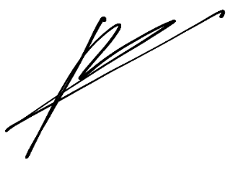
\includegraphics[height=1.8cm, width=3.5cm, keepaspectratio]{pic/rizkiafdl_signature.png} &
        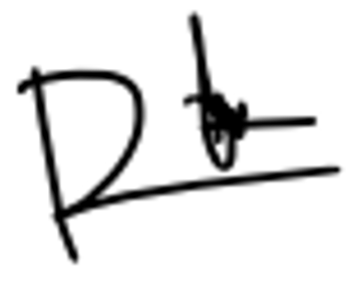
\includegraphics[height=1.8cm, width=3.5cm, keepaspectratio]{pic/rakha_picture.png} &
        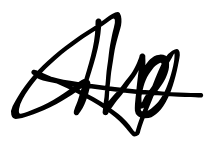
\includegraphics[height=1.8cm, width=3.5cm, keepaspectratio]{pic/ttdtheo.png} \\[4pt]

        \underline{\makebox[3.8cm][c]{\penulisSatu}} & \underline{\makebox[3.8cm][c]{\penulisDua}} & \underline{\makebox[3.8cm][c]{\penulisTiga}} \\[4pt]

        \fontsize{12}{14}\selectfont\bf{\NIMpenulisSatu} & \fontsize{12}{14}\selectfont\bf{\NIMpenulisDua} & \fontsize{12}{14}\selectfont\bf{\NIMpenulisTiga} \\

        \end{tabular}

        \vspace*{0.7 cm}
        % \bo{{\Type}}  \\
        % \vspace*{0.7 cm}

        \bo{Disetujui oleh}:\\
        \bo{Pembimbing dan Head of Study Program}\\
\end{center}

    % \vspace{\baselineskip}
    \vspace{1.5cm}
        
    \begin{center}
    \begin{minipage}{12cm}
        \centering
        % \hrulefill\\
        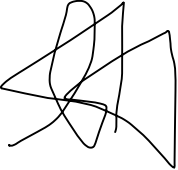
\includegraphics[height=1.8cm, width=5.5cm, keepaspectratio]{pic/pak_budi_signature.png}\\[4pt]
        \underline{\pembimbingSatu} \\[4pt]
        \fontsize{12}{14}\selectfont\bf{\nikSatu}\\
    \end{minipage}
    \end{center}

    % \vspace{1.5cm}
    % \renewcommand{\arraystretch}{0.7} 
    % \begin{center}
    %     \begingroup
    %     \begin{tabular}{ccc}
    %     % \hrulefill & & \hrulefill \\
    %     \underline{\pembimbingDua} & & \underline{\pembimbingTiga} \\
    %     \fontsize{12}{0}\bf{KO-PROMOTOR 1} & & \fontsize{12}{0}\bf{KO-PROMOTOR 2}\\
    %     \end{tabular}
    % \end{center}

    % \begin{center}\setstretch{2.0}{Mengetahui,}\end{center}

    \vspace{2cm}
    % \begin{center}
    %     \begin{minipage}{10cm}
    %     \centering
    %     % \hrulefill\\
    %     % \underline{\pembimbingDua}  \\[4pt]
    %     % \fontsize{12}{14}\selectfont\bf{Head of Computer Science Study Program}\\
    %     \end{minipage}
    % \end{center}

 
  
    

% PERNYATAAN
% \chapter*{}
\thispagestyle{plain}
    % \vspace*{-3cm}
    % \noindent Halaman Pernyataan Orisinalitas 
% \justifying{\noindent\textbf{Halaman Persetujuan Publikasi Skripsi}}

% \vspace*{1cm}
\centering{\large{\bo{PERNYATAAN}}}
\vspace*{.5cm}

\justifying
\noindent Dengan ini saya, \\

\renewcommand{\arraystretch}{1} % Catatan: Ubah ke 1.5 jika ingin tinggi baris bertambah 50%. Kalau angka 1 itu kembali ke ukuran normal.
\noindent % Menghilangkan indentasi otomatis pada tabel agar sejajar dengan teks di atasnya
\begin{tabular}{l c p{0.65\textwidth}}
Nama          & : & \penulis \\
NIM           & : & \nim \\
Judul Skripsi & : & \Judul \\
\end{tabular}

\vspace*{1 cm}
Memberikan kepada Universitas Bina Nusantara hak non-eksklusif untuk menyimpan, memperbanyak, dan menyebarluaskan Skripsi karya saya, secara keseluruhan atau hanya sebagian atau hanya ringkasannya saja, dalam bentuk format tercetak dan atau elektronik.

% \vspace*{1 cm}
Menyatakan bahwa saya, akan mempertahankan \textbf{hak eksklusif} saya, untuk menggunakan seluruh atau sebagian isi Skripsi saya, guna pengembangan karya di masa depan, misalnya bentuk artikel, buku, perangkat lunak, ataupun sistem informasi. \\

% \noindent Jakarta, \today \\
% \noindent Hormat Saya, \\

% \begin{flushright}
% Jakarta, \tanggalPengesahan\\[0.1cm]
% \vspace*{1cm}
% \penulis

% \end{flushright}

% --- Mulai Area Tanda Tangan ---

\noindent % Pastikan baris ini dimulai dari paling kiri
Jakarta, \tanggalPengesahan,\\
\begin{tabular}{p{0.45\textwidth} p{0.45\textwidth}}
    % --- KOLOM KIRI ---
    \raggedright % Konten di kolom ini rata tengah
    
    \noindent Hormat Saya,
    \vspace{2cm} \newline % Beri jarak dan baris baru
    \underline{\textbf{\penulis}} \\[-6pt]
    \nim
    
    & % Pindah ke kolom kanan
    
    % --- KOLOM KANAN ---
    \raggedright % Konten di kolom ini rata tengah
                  % \\
    Diketahui oleh
    \vspace{2cm} \newline % Beri jarak dan baris baru
    \underline{\textbf{\pembimbingSatu}} \\[-6pt]
    D6408
\end{tabular}

% --- Akhir Area Tanda Tangan ---

% Kata Pengantar
% \addChapter{\kataPengantar}
% \addcontentsline{toc}{section}{Kata Pengantar}
%-----------------------------------------------------------------------------%
% \chapter*{\kataPengantar}
% \contentsname*{\kataPengantar}
% \addcontentsline{toc}{section}{{Kata Pengantar}}
\addcontentsline{toc}{section}{Kata Pengantar}
\thispagestyle{plain}
%-----------------------------------------------------------------------------%
\section*{\centering{\large{KATA PENGANTAR}}}
\justifying
\setstretch{1.5}{
% {\bf \textit{(Not limited to this, this is only example; students should not copy exactly by words)}}\\\\
    Puji syukur kepada Tuhan Yang Maha Esa dengan selesainya XXX dengan judul \JudulIndo. Penulis mengucapkan terima kasih yang sedalam-dalamnya kepada berbagai pihak yang telah memberikan masukan, bimbingan, arahan, dan semangat dalam mengerjakan XXX ini, yaitu kepada:
        
    \begin{enumerate}
        \item Ibu Dr. Nelly, S.Kom., M.M., CSA. selaku Rektor Universitas Bina Nusantara Periode 2023 – 2028.
        \item xxx selaku Direktur BINUS Bandung.
        \item xxx selaku Head of Department of Computer Science, Universitas Bina Nusantara.
        \item \lipsum*[1][1]
        \item Pihak lain yang tidak dapat disebutkan satu persatu.
    \end{enumerate}
        
    Akhir kata, kiranya segala bimbingan, saran, dan masukan dari Bapak/Ibu yang telah diberikan kepada penulis, akan mendapat berkah dari Tuhan Yang Maha Esa.
	}
\vspace*{0.1cm}
\begin{flushright}
Jakarta, \tanggalPengesahan\\[0.1cm]
\vspace*{1cm}
\penulis

\end{flushright}

% Abstrak Bahasa Indonesia dan Bahasa Iggris
% \addChapter{ABSTRAK}
% \chapter*{Abstrak}
\addcontentsline{toc}{section}{Abstrak}
\thispagestyle{plain}

% \vspace*{0.3 cm}
% \lipsum[1] \par
% \vspace*{1 cm}
\begin{center}
    \textbf{UNIVERSITAS BINA NUSANTARA}\\
    % % \vspace*{1 cm}
    % \textbf{Pernyataan Kesiapan Skripsi untuk Ujian Pendadaran}
\end{center}

\begin{center}
Computer Science Study Program \\
School of Computer Science \\
Skripsi Sarjana Teknik Informatika \\
\end{center}

\begin{center}
    \bo{{\JudulIndo}} \\
    \vspace*{0.5 cm}
    \penulisSatu - \NIMpenulisSatu \\
    \penulisDua - \NIMpenulisDua \\
    \penulisTiga - \NIMpenulisTiga \\
\end{center}

\begin{center}
    \textbf{\textit{ABSTRACT}}
\end{center}

\lipsum[1] \par
\textit{\noindent\textbf{Keywords}: keyword1, keyword2, xxx.}

\begin{center}
    \textbf{ABSTRAK}
\end{center}

\lipsum[1] \par

\textit{\noindent\textbf{Keywords}: keyword1, keyword2, xxx.}


% 
\chapter*{ABSTRACT}
\addcontentsline{toc}{section}{Abstract}
\thispagestyle{plain}

\vspace*{0.7cm}
\lipsum[1]
\vspace*{1 cm}

\textit{\noindent\textbf{Keywords}: keyword1, keyword2, xxx.}
\newpage
\newpage



% \addChapter{UCAPAN TERIMA KASIH}
% \include{ucapan}

% % Daftar isi, gambar, dan tabel
\tableofcontents
\addcontentsline{toc}{section}{Daftar Isi}
\renewcommand\contentsname{Daftar Isi}
\clearpage

\listoffigures
\addcontentsline{toc}{section}{Daftar Gambar}
\renewcommand{\listfigurename}{Daftar Gambar}
\clearpage

\listoftables
\addcontentsline{toc}{section}{Daftar Tabel}
\renewcommand{\listtablename}{Daftar Tabel}
\clearpage

% \addChapter{DAFTAR SINGKATAN}
% \include{singkatan}

% \addChapter{DAFTAR SIMBOL}
% \include{simbol}

% \addChapter{DAFTAR ISTILAH}
% \chapter*{DAFTAR ISTILAH}

\begin{center}
	\centering
	\begin{tabular}{p{2cm}p{12cm}}
		\textit{Transmitter} &: Pemancar \\
		\textit{Receiver} & Penerima sinyal\\
		
		
		
	\end{tabular}
\end{center}

% % Daftar Lampiran
% \addChapter{DAFTAR LAMPIRAN}
% \include{listofappendix}

%Comment disini%

% Gunakan penomeran Arab (1, 2, 3, ...) setelah bagian ini.
\pagenumbering{arabic}
\pagestyle{mainstyle}  % <--- TAMBAHKAN BARIS INI
% Bab 1 : Pendahuluan
\chapter{\babSatu}



\section{Latar Belakang}\label{latar-belakang}

Program Enrichment merupakan bagian dari kurikulum Universitas XYZ yang memberi mahasiswa pengalaman pembelajaran berbasis praktik. Program ini terbagi ke dalam beberapa jalur, dan penelitian ini difokuskan pada jalur magang (\textit{internship}). Selama menjalani jalur magang, setiap mahasiswa didampingi oleh seorang Faculty Supervisor yang bertugas memberikan arahan akademik, memantau perkembangan, serta mengevaluasi mahasiswa sepanjang periode program. Karena pendampingan ini memengaruhi capaian pembelajaran mahasiswa, kesesuaian bidang keahlian antara mahasiswa dan Faculty Supervisor menjadi pertimbangan yang menentukan mutu bimbingan.

Penugasan Faculty Supervisor saat ini masih ditangani secara manual. Berdasarkan wawancara terstruktur bersama Margareth Setiawan, Yulianto, dan Mila Andria Savitri selaku \textit{Enrichment Program Coordinator} (EPC) dari tiga fakultas di XYZ University pada 13 Desember 2025, pemetaan mahasiswa ke Faculty Supervisor dikerjakan menggunakan \textit{spreadsheet}. Untuk satu \textit{batch} yang dapat mencapai ratusan mahasiswa, proses ini memakan waktu satu hingga tiga minggu dan kerap disertai revisi berulang hingga dua puluh kali per \textit{batch} akibat kesalahan penempatan. Penetapan pembimbing pun cenderung dilakukan tanpa mempertimbangkan kesesuaian bidang keahlian, sehingga sebagian mahasiswa memperoleh Faculty Supervisor yang kurang relevan dengan topik magangnya.

Cara kerja manual ini membawa beberapa akibat. Beban bimbingan antardosen menjadi tidak merata karena tidak ada acuan kuota, sebagian mahasiswa ditempatkan di luar bidang keahlian pembimbingnya, dan setiap kesalahan penempatan menuntut EPC menyunting ulang data secara manual. Hal-hal tersebut menambah beban kerja EPC dan menyulitkan penelusuran alasan di balik setiap penempatan.

\begin{figure}[h]
\centering
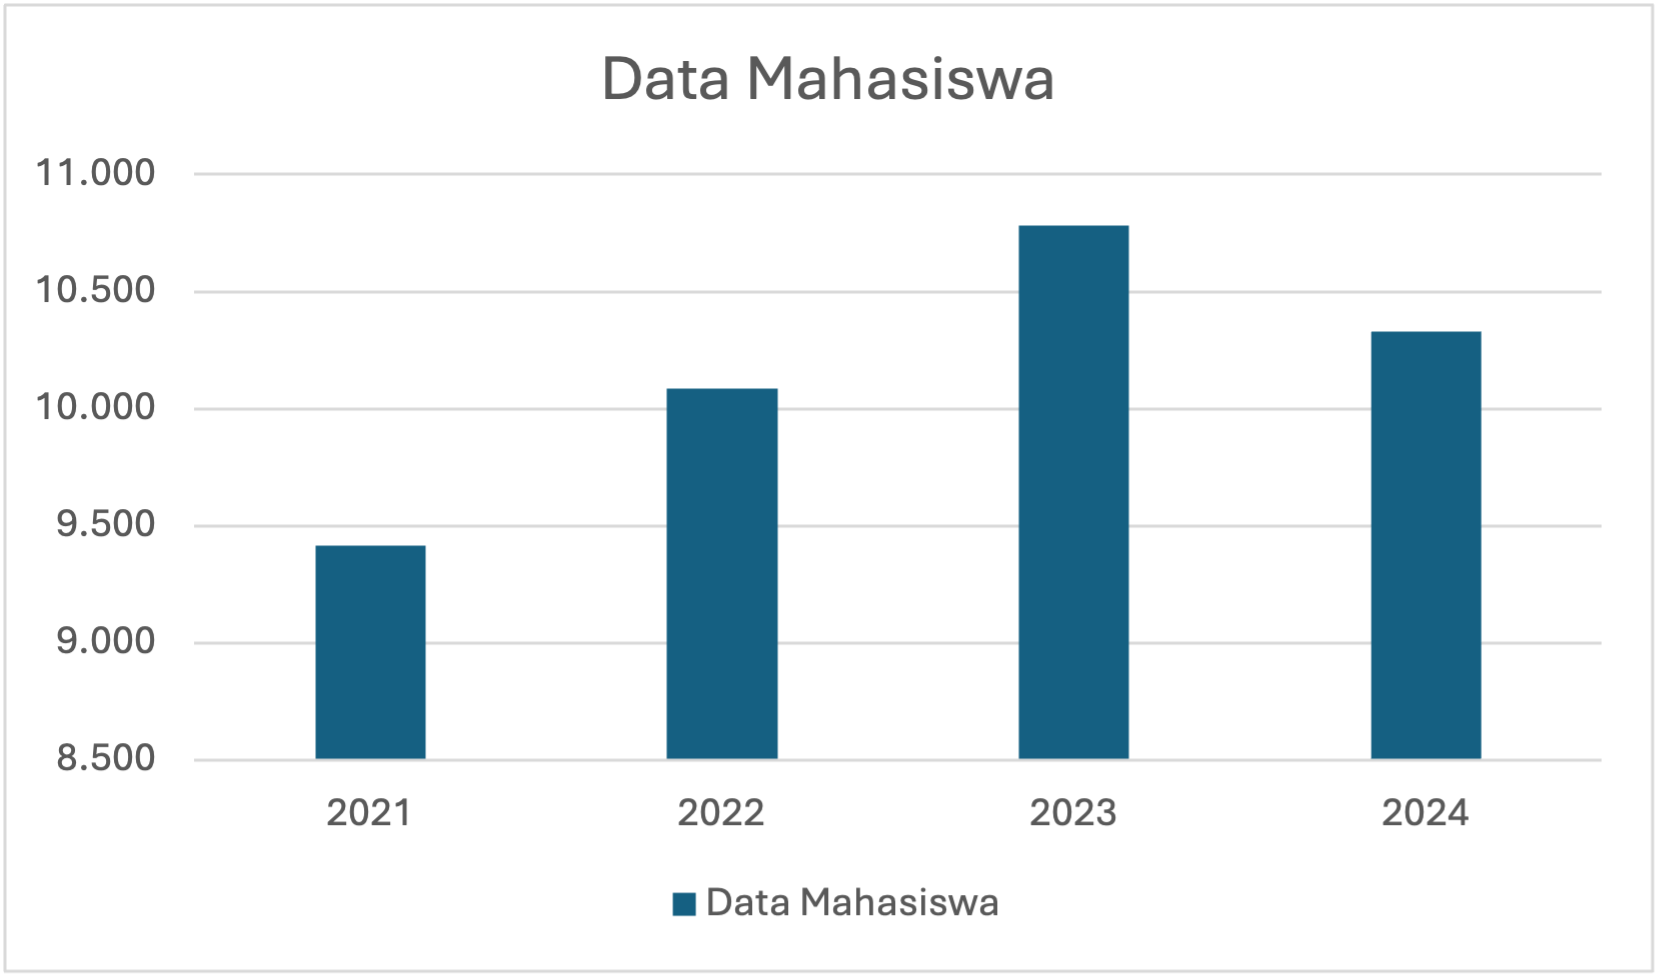
\includegraphics[width=0.85\linewidth]{pic/pertumbuhan-mahasiswa}
\caption{Pertumbuhan Jumlah Mahasiswa XYZ University Tahun 2021--2025}
\label{fig:fig1.1}
% {\footnotesize Sumber: Diolah dari \cite{binusmaba2021}, \cite{binusmaba2022}, \cite{binusmaba2023}, \cite{binusmaba2024}, \cite{binusmaba2025}}
\end{figure}

Beban proses ini bertambah seiring meningkatnya jumlah mahasiswa XYZ University pada periode 2021--2025 sebagaimana ditunjukkan Gambar~\ref{fig:fig1.1}, yang berdampak pula pada bertambahnya peserta Program Enrichment yang harus dipetakan. Dengan volume data yang lebih besar, pemetaan manual makin sulit dijaga konsistensi dan kecepatannya. Penelitian ini mengusulkan sistem rekomendasi berbasis \textit{semantic similarity} untuk membantu EPC, yaitu pendekatan yang mengukur kesesuaian antara profil mahasiswa dan bidang keahlian dosen dari kemiripan makna data tekstual keduanya.

Upaya mengotomasi alokasi pembimbing akademik telah dilakukan pada sejumlah penelitian. Evangelista, Fan, dan Harb (\citeyear{fan2021automated}) menunjukkan bahwa pendekatan otomatis berbasis \textit{machine learning} dapat mengatasi keterbatasan pemetaan manual, terutama pada institusi berjumlah mahasiswa besar. Pada konteks yang lebih dekat, Rismanto, Syulistyo, dan Agusta (\citeyear{rismanto2020supervisor}) membangun sistem rekomendasi dosen pembimbing tugas akhir dengan pembobotan TF-IDF dan \textit{cosine similarity} yang mencapai akurasi rata-rata 75\% terhadap data aktual. Kelemahannya, TF-IDF mencocokkan kata kunci secara leksikal sehingga gagal mengenali kesamaan makna ketika mahasiswa dan dosen memakai istilah berbeda untuk topik yang serupa. Untuk mengatasi keterbatasan itu, penelitian ini menempuh pendekatan \textit{semantic similarity} dengan model \textit{embedding} yang menilai kesesuaian profil mahasiswa dan bidang keahlian Faculty Supervisor berdasarkan makna teks, bukan sekadar kecocokan kata.

Kualitas rekomendasi diukur dengan membandingkan keluaran sistem terhadap \textit{ground truth}. Pada penelitian ini, \textit{ground truth} berasal dari data institusional penugasan \textit{faculty supervisor} \textit{batch} 2026 Program Enrichment program studi Computer Science di XYZ University. Data tersebut disiapkan oleh EPC dan memuat penugasan aktual (\texttt{current\_supervisor\_code}) hasil pemetaan manual yang benar-benar diterapkan pada periode itu, sehingga mewakili praktik penentuan Faculty Supervisor yang berlaku secara institusional.

Sistem yang dikembangkan diposisikan sebagai \textit{decision support system}: keluarannya berupa rekomendasi bagi EPC, sedangkan keputusan akhir tetap ditetapkan oleh EPC. Metode yang diusulkan diwujudkan dalam sebuah prototipe berupa antarmuka pengguna dengan \textit{backend} sederhana, dan dibatasi pada jalur magang Program Enrichment program studi Computer Science di XYZ University kampus Bandung. Dengan bantuan sistem ini, EPC diharapkan dapat memetakan Faculty Supervisor lebih cepat dan dengan dasar pertimbangan yang dapat ditelusuri.

\section{Rumusan Masalah}\label{rumusan-masalah}

Berdasarkan latar belakang yang telah diuraikan, rumusan masalah dalam penelitian ini adalah sebagai berikut:

\begin{enumerate}
\def\labelenumi{\arabic{enumi}.}
\item
  Bagaimana merancang dan mengembangkan sistem rekomendasi Faculty Supervisor magang berbasis \textit{semantic similarity}?
\item
  Seberapa tinggi tingkat kesesuaian hasil rekomendasi sistem dengan \textit{ground truth} yang diperoleh dari pencocokan manual oleh EPC?
\item
  Bagaimana sistem rekomendasi yang dikembangkan dapat membantu meningkatkan efisiensi proses pemetaan Faculty Supervisor magang oleh EPC?
\end{enumerate}

\section{Ruang Lingkup Penelitian}\label{ruang-lingkup-penelitian}

Agar penelitian ini lebih terarah, ruang lingkup penelitian dibatasi pada:

\begin{enumerate}
\def\labelenumi{\arabic{enumi}.}
\item
  Penelitian difokuskan pada pemetaan Faculty Supervisor magang dalam Program Enrichment di XYZ University kampus Bandung, khususnya pada program studi Computer Science.
\item
  Sistem rekomendasi dikembangkan menggunakan pendekatan \textit{semantic similarity} berbasis data tekstual.
\item 
  Data yang digunakan dalam penelitian ini dibatasi pada data \textit{enrichment} \textit{batch} 2026 yang memuat data mahasiswa peserta Program \textit{Enrichment}, data \textit{Faculty Supervisor}, serta data institusional penugasan \textit{faculty supervisor} sebagai \textit{ground truth}.
\item 
  Website memiliki fitur utama berupa halaman beranda, \textit{data center} untuk pengelolaan data mahasiswa, \textit{run history} untuk melihat hasil rekomendasi sebelumnya, serta halaman \textit{supervisor studio} untuk melihat profil dosen dan kata kunci yang diterapkan.
\item
  Evaluasi sistem dilakukan dengan membandingkan hasil rekomendasi dengan \textit{ground truth} yang diperoleh dari data institusional penugasan \textit{faculty supervisor} Program Enrichment.
\item
  Penelitian menghasilkan sebuah prototipe sistem yang mencakup antarmuka pengguna dan \textit{backend}.
\item
  Penelitian ini tidak membahas kebijakan akademik di luar proses pemetaan Faculty Supervisor.
\item 
  Pengujian sistem menggunakan metode \textit{black box}, untuk fungsionalitas yang dihasilkan, tanpa membahas detail implementasi teknis secara mendalam.
\item
  Penelitian ini tidak mencakup evaluasi usabilitas atau penerimaan pengguna oleh EPC; pengujian dilakukan terbatas pada validasi fungsionalitas sistem.

\end{enumerate}
\section{Tujuan dan Manfaat}\label{tujuan-dan-manfaat}

\subsection{Tujuan}\label{tujuan}

Tujuan dari penelitian ini adalah sebagai berikut:

\begin{enumerate}
\def\labelenumi{\arabic{enumi}.}
\item
  Menganalisis permasalahan dalam proses pemetaan Faculty Supervisor Program Enrichment yang dilakukan secara manual.
\item
  Mengembangkan sistem rekomendasi Faculty Supervisor magang menggunakan pendekatan \textit{semantic similarity}.
\item
  Melakukan evaluasi hasil rekomendasi sistem menggunakan \textit{ground truth} berdasarkan pencocokan manual.
\item
  Menghasilkan prototipe sistem sebagai pendukung EPC dalam proses penentuan Faculty Supervisor secara lebih efektif dan terstruktur.
\end{enumerate}

\subsection{Manfaat}\label{manfaat}

Adapun manfaat yang diharapkan dari pengembangan sistem ini adalah:

\begin{enumerate}
\def\labelenumi{\arabic{enumi}.}
\item
  Membantu EPC dalam mempercepat dan mempermudah proses pemetaan mahasiswa ke Faculty Supervisor.
\item
  Mengurangi kesalahan dan revisi pemetaan yang disebabkan oleh proses manual.
\item
  Meningkatkan kesesuaian antara minat mahasiswa dan bidang keahlian Faculty Supervisor.
\item
  Menjadi dasar pengembangan sistem pemetaan Faculty Supervisor yang lebih terintegrasi di masa depan.
\end{enumerate}

\section{Metode Penelitian}\label{metode-penelitian}

Metode penelitian disusun untuk mendukung pengembangan sistem rekomendasi Faculty Supervisor magang pada Program Enrichment XYZ University. Penelitian menggunakan pendekatan rekayasa perangkat lunak dengan \textit{semantic similarity} sebagai dasar mekanisme rekomendasi, dan hasilnya dievaluasi terhadap \textit{ground truth} dari pencocokan manual EPC.

Tahapan metode penelitian secara umum meliputi studi pustaka, pengumpulan data, praproses data, pengembangan sistem rekomendasi, evaluasi sistem, serta pengembangan prototipe sistem.

\subsection{Pengumpulan Data}\label{pengumpulan-data}

Pengumpulan data dilakukan melalui studi dokumen dan data institusional yang digunakan dalam proses pemetaan Faculty Supervisor Program Enrichment. Data yang digunakan meliputi data Faculty Supervisor, data mahasiswa peserta jalur magang Program Enrichment, serta dokumen pemetaan historis Faculty Supervisor dan mahasiswa dalam rentang waktu satu tahun terakhir di XYZ University. Data \textit{ground truth} diperoleh dari data institusional penugasan \textit{faculty supervisor} \textit{batch} 2026 Program Enrichment program studi Computer Science di XYZ University, yang memuat atribut penugasan aktual (\texttt{current\_supervisor\_code}) hasil pemetaan manual EPC.

\subsection{Metode Perancangan Sistem}

Pada tahap ini dilakukan perancangan sistem menggunakan pendekatan \textit{System Development Life Cycle} (SDLC) dengan model \textit{Waterfall}. Proses ini dilakukan secara terstruktur dan sekuensial yang meliputi beberapa tahapan utama sesuai dengan jadwal kegiatan penelitian, yaitu analisis masalah dan kebutuhan sistem, perancangan sistem (menggunakan \textit{Unified Modeling Language} dan arsitektur sistem), pengembangan sistem atau implementasi kode, pengujian dan evaluasi sistem, serta diakhiri dengan tahap revisi dan finalisasi dokumen.

\subsection{Praproses Data}\label{praproses-data}

Sebelum data digunakan dalam sistem rekomendasi, data tekstual melewati tahap praproses untuk menjaga konsistensi. Tahap ini mencakup penyeragaman huruf (\textit{case folding}), pembersihan karakter yang tidak relevan, dan normalisasi spasi. Praproses sengaja dibuat ringkas karena model \textit{embedding} berbasis \textit{transformer} sudah menangani variasi morfologi melalui tokenisasi \textit{subword}, sehingga langkah agresif seperti \textit{stemming} dihindari agar sinyal makna tidak terbuang.

\subsection{Pengembangan Sistem Rekomendasi}\label{pengembangan-sistem-rekomendasi}

Inti sistem adalah perhitungan \textit{semantic similarity} antara profil mahasiswa dan bidang keahlian Faculty Supervisor. Data tekstual keduanya diubah menjadi representasi vektor melalui model \textit{embedding}, lalu kemiripannya dihitung untuk menyusun peringkat rekomendasi Faculty Supervisor bagi setiap mahasiswa.

Di atas perhitungan kemiripan semantik, sistem menerapkan aturan pendukung berupa batasan kuota per Faculty Supervisor agar beban pembimbing lebih merata. Rekomendasi yang dihasilkan berperan sebagai bahan pertimbangan EPC; keputusan akhir tetap ditetapkan oleh EPC sesuai posisi sistem sebagai \textit{decision support system}.

\subsection{Pengembangan Prototipe Sistem}\label{pengembangan-prototipe-sistem}

Metode yang diusulkan diwujudkan dalam prototipe berupa antarmuka pengguna dengan \textit{backend} sederhana. Prototipe ini menjalankan alur kerja rekomendasi dari \textit{input} data, perhitungan kemiripan, hingga penyajian hasil kepada EPC, sehingga metode dapat diuji dalam bentuk sistem yang berjalan, bukan sekadar rancangan.

\subsection{Evaluasi Sistem}\label{evaluasi-sistem}

Evaluasi sistem dilakukan dengan membandingkan hasil rekomendasi yang dihasilkan oleh sistem dengan \textit{ground truth} yang diperoleh dari data institusional penugasan \textit{faculty supervisor} Program Enrichment. Evaluasi ini bertujuan untuk menilai tingkat kesesuaian dan relevansi rekomendasi sistem terhadap keputusan manual yang telah diterapkan. Hasil evaluasi digunakan untuk menganalisis kinerja sistem serta potensi peningkatan efektivitas proses pemetaan Faculty Supervisor.

\section{Sistematika Penulisan}\label{sistematika-penulisan}

Skripsi ini disusun dengan sistematika penulisan yang terdiri dari lima bab dengan rincian sebagai berikut:

\textbf{BAB 1 PENDAHULUAN}

Bab ini membahas latar belakang permasalahan, rumusan masalah, ruang lingkup, tujuan dan manfaat, metode penelitian, hingga sistematika penulisan yang digunakan.

\textbf{BAB 2 TINJAUAN PUSTAKA}

Bab ini berfokus pada pembahasan teori-teori yang berkaitan dengan sistem rekomendasi, \textit{semantic similarity}, \textit{natural language processing}, serta penelitian terdahulu yang relevan sebagai dasar pengembangan sistem.

\textbf{BAB 3 METODE PENELITIAN}

Bab ini memberikan penjelasan mengenai metode penelitian yang digunakan pada penelitian ini, tahapan pengembangan sistem rekomendasi, arsitektur sistem, serta perancangan alur dan komponen sistem.

\textbf{BAB 4 HASIL DAN PEMBAHASAN}

Bab ini membahas proses implementasi sistem rekomendasi, hasil pengujian sistem, serta analisis dan pembahasan hasil evaluasi yang diperoleh.

\textbf{BAB 5 SIMPULAN DAN SARAN}

Bab ini membahas mengenai kesimpulan dan saran - saran yang diusulkan dari hasil penelitian yang dilakukan dalam tugas akhir agar dapat dikembangkan lebih lanjut kedepannya




% % Bab 2 : Dasar Teori
%-----------------------------------------------------------------------------%
\chapter{\babDua}
%\begin{center}
%	\textbf{BAB II}
%	\par \textbf{TINJAUAN PUSTAKA}
%\end{center}
%---------------------------------------------------------------------------%-----------------------------------------------------------------------------%
\lipsum[1]. Mensitasi \cite{article} atau  \citep{article}. Teori ini diteliti oleh \cite{deepfake-1}. Di mana \(v\) adalah kecepatan \citep{deepfake-1}.

\section{Sub bab pertama}
\lipsum[1]

\begin{figure}[tp!]
		\centering	
		
\includegraphics[width=1\linewidth]{pic/logo.png}
		\caption{Caption gambar}
        \label{fig:fig2.1}
\end{figure}

\section{Sub bab kedua}
\lipsum[1]

\subsection{Sub sub bab pertama}
\lipsum[1]

\section{Sub bab ketiga} 
\lipsum[1]

\begin{table}[tp!]
\renewcommand{\arraystretch}{1}
	\caption{Caption Tabel.}
	\label{table:tab2.4}
\centering
\begin{tabular}{|>{\fontsize{11}{14}\selectfont}p{2cm}|>{\fontsize{11}{14}\selectfont}p{5cm}|>{\fontsize{11}{14}\selectfont}p{2cm}|>{\fontsize{11}{14}\selectfont}p{3cm}|}
    \hline
    \textbf{Kolom 1} & \textbf{Kolom 2} & \textbf{Kolom 3} & \textbf{Kolom 4} \\
    \hline
    lorem ipsum & lorem ipsum. & lorem ipsum & \cite{article} \\
    \hline
    lorem ipsum & lorem ipsum. & lorem ipsum & \cite{article} \\
    \hline
\end{tabular}
\end{table}

Menulis angka $92,62\%$ dan $90,79\%$. 






% % Bab 3 : Perancangan
%-----------------------------------------------------------------------------%
\chapter{\babTiga}
%\begin{center}
%	\textbf{BAB III}
%	\par \textbf{PERENCANAAN SISTEM}
%\end{center}
%-----------------------------------------------------------------------------%
\textit{Satu paragraf menjelaskan isi bab tiga}. \lipsum[1]

\section{Sub bab pertama}
\lipsum[1]

Membuat persamaan \ref{equation-bab-3}

\begin{equation}\label{equation-bab-3}
    \begin{gathered}b=\begin{cases}1,&I(\mathbf{p}^{\alpha }_{j} ,\sigma_{j} )>I(\mathbf{p}^{\alpha }_{i} ,\sigma_{i} )\\ 0,&\text{otherwise} \end{cases} \\ \forall (\mathbf{p}^{\alpha }_{j} ,\sigma_{j} )\in \zeta \end{gathered}  
\end{equation}



% % Bab 4 : Pengujian
%-----------------------------------------------------------------------------%
\chapter{\babEmpat}
%\begin{center}
%	\textbf{BAB IV}
%	\par \textbf{ANALISIS SIMULASI SISTEM}
%\end{center}
%-----------------------------------------------------------------------------%

\section{Testing Environment}
Dalam penelitian ini, penulis menggunakan bahasa pemrograman Python untuk membangun dan mengimplementasikan sistem rekomendasi Faculty Supervisor berbasis semantic similarity. Penulis juga menggunakan perangkat keras dan lunak tertentu untuk mengembangkan sistem tersebut. Berikut adalah daftar perangkat keras yang digunakan dalam penelitian ini.
\begin{table}

\centering
\begin{tabular}{|>{\fontsize{11}{14}\selectfont}p{2cm}|>{\fontsize{11}{14}\selectfont}p{5cm}|>{\fontsize{11}{14}\selectfont}p{2cm}|>{\fontsize{11}{14}\selectfont}p{3cm}|}
    \hline
    \textbf{Komponen} & \textbf{Spesifikasi} \\
    \hline
    Processor & Apple M4 Pro (12-core CPU) \\ 
    \hline
    RAM & 24 GB Unified Memory  \\
    \hline
    GPU & Apple M4 Pro Integrated GPU (20-core) + Apple Neural Engine (16-core)  \\
    \hline
    Disk Space & 1 TB SSD \\
    \hline
\end{tabular}
\renewcommand{\arraystretch}{1}
	\caption{Spesifikasi Perangkat Keras}
	\label{table:tab4.1}
\end{table}

Perangkat keras tersebut juga menggunakan beberapa perangkat lunak untuk proses pengembangan sistem rekomendasi Faculty Supervisor. Spesifikasi perangkat lunak yang digunakan adalah sebagai berikut. 

\begin{table}
 \centering
\begin{tabular}{|>{\fontsize{11}{14}\selectfont}p{2cm}|>{\fontsize{11}{14}\selectfont}p{5cm}|>{\fontsize{11}{14}\selectfont}p{2cm}|>{\fontsize{11}{14}\selectfont}p{3cm}|}
    \hline
    \textbf{Komponen} & \textbf{Spesifikasi} \\
    \hline
    Sistem Operasi & macOS Sequoia 15  \\ 
    \hline
    Bahasa Pemrograman  & Python 3.12   \\
    \hline
    Web Framework  & Flask 3.1.0   \\
    \hline
    ORM ; Database  & SQLAlchemy 2.0.49 + SQLite  \\
    \hline
    Embedding Library  & sentence-transformers   \\
    \hline
    Model Kandidat   & BAAI/bge-m3, Qwen/Qwen3-Embedding-0.6B, intfloat/multilingual-e5-large-instruct   \\
    \hline
    Data Processing    & pandas, numpy, openpyxl    \\
    \hline
   IDE    & Visual Studio Code   \\
    \hline
\end{tabular}
\renewcommand{\arraystretch}{1}
	\caption{Spesifikasi Perangkat Lunak}
	\label{table:tab4.2}
\end{table}

\section{Hasil}
\subsection{Evaluasi Model}

Pada tahap ini dilakukan evaluasi terhadap tiga model \textit{embedding} yang menjadi kandidat untuk komponen perhitungan kemiripan semantik. Seluruh model dievaluasi menggunakan \textit{pipeline}, dataset, serta konfigurasi kapasitas yang identik agar perbandingan bersifat adil; satu-satunya variabel yang diubah adalah model \textit{embedding} yang digunakan. Untuk memastikan keterulangan (\textit{reproducibility}), seluruh proses dibuat deterministik sehingga eksekusi berulang menghasilkan keluaran yang identik.

Evaluasi dilakukan terhadap \textbf{168 dari 171 mahasiswa}. Sebanyak 3 mahasiswa dikecualikan karena tidak memiliki nilai \texttt{current\_supervisor\_code} yang valid sebagai \textit{ground truth}.

Pengukuran dilakukan pada dua tingkat yang saling melengkapi:

\begin{itemize}
    \item \textbf{Metrik \textit{retrieval} (sebelum \textit{solver}):} MRR, Hit@1, Hit@5, NDCG@5, NDCG@10, dan rata-rata peringkat (\textit{avg\_rank}). Metrik ini mengukur kualitas pemeringkatan dosen pembimbing sebelum proses alokasi kapasitas dijalankan.
    \item \textbf{Metrik \textit{assignment} (setelah \textit{solver}):} \textit{Assignment Match Rate}. Metrik ini mengukur kesesuaian hasil penugasan akhir terhadap penugasan historis admin.
\end{itemize}

Hasil evaluasi seluruh model kandidat disajikan pada Tabel~\ref{table:tab4.2.1}.

\begin{table}[h]
\centering
\begin{tabular}{|>{\fontsize{9}{12}\selectfont}p{3.2cm}|>{\fontsize{9}{12}\selectfont}p{1.2cm}|>{\fontsize{9}{12}\selectfont}p{1.2cm}|>{\fontsize{9}{12}\selectfont}p{1.2cm}|>{\fontsize{9}{12}\selectfont}p{1.2cm}|>{\fontsize{9}{12}\selectfont}p{1.4cm}|>{\fontsize{9}{12}\selectfont}p{1.4cm}|>{\fontsize{9}{12}\selectfont}p{1.4cm}|}
    \hline
    \textbf{Model} & \textbf{MRR} & \textbf{Hit@1} & \textbf{Hit@5} & \textbf{NDCG@5} & \textbf{NDCG@10} & \textbf{Avg Rank} & \textbf{Match Rate} \\
    \hline
    \textbf{BAAI/bge-m3} (Run 5) & 0,585 & 0,417 & 0,804 & 0,622 & 0,668 & 3,32 & 0,357 \\
    \hline
    \textbf{Qwen/Qwen3-Embedding-0.6B} (Run 6) & 0,474 & 0,298 & 0,708 & 0,505 & 0,576 & 4,20 & 0,357 \\
    \hline
    \textbf{intfloat/multilingual-e5-large-instruct} (Run 9) & 0,469 & 0,304 & 0,649 & 0,483 & 0,563 & 4,60 & 0,381 \\
    \hline
    \textit{Random baseline} & $\sim$0,23 & $\sim$0,07 & $\sim$0,36 & $\sim$0,21 & --- & $\sim$7,5 & --- \\
    \hline
\end{tabular}
\renewcommand{\arraystretch}{1}
    \caption{Perbandingan Metrik Evaluasi Antar Model}
    \label{table:tab4.2.1}
\end{table}

Secara deskriptif, \textbf{BAAI/bge-m3} memperoleh MRR sebesar 0,585 dengan dosen pembimbing sebenarnya berada pada peringkat rata-rata 3,32. \textbf{Qwen/Qwen3-Embedding-0.6B} memperoleh MRR 0,474 dengan rata-rata peringkat 4,20. \textbf{intfloat/multilingual-e5-large-instruct} memperoleh MRR 0,469 dengan rata-rata peringkat 4,60, namun memiliki \textit{Assignment Match Rate} tertinggi sebesar 0,381. Seluruh model berada jauh di atas \textit{random baseline}, yang menunjukkan bahwa pendekatan kemiripan semantik memberikan sinyal pencocokan yang nyata.

Untuk keperluan analisis lebih lanjut, nilai rata-rata skor kemiripan disajikan pada Tabel~\ref{table:tab4.2.2}.

\begin{table}[h]
\centering
\begin{tabular}{|>{\fontsize{11}{14}\selectfont}p{3.5cm}|>{\fontsize{11}{14}\selectfont}p{3cm}|>{\fontsize{11}{14}\selectfont}p{3cm}|>{\fontsize{11}{14}\selectfont}p{2.5cm}|}
    \hline
    \textbf{Model} & \textbf{Avg Similarity @1} & \textbf{Avg True Similarity} & \textbf{Selisih (sebaran)} \\
    \hline
    \textbf{BAAI/bge-m3} (Run 5) & 0,619 & 0,596 & 0,023 \\
    \hline
    \textbf{Qwen/Qwen3-Embedding-0.6B} (Run 6) & 0,692 & 0,624 & 0,068 \\
    \hline
    \textbf{intfloat/multilingual-e5-large-instruct} (Run 9) & 0,871 & 0,857 & 0,014 \\
    \hline
\end{tabular}
\renewcommand{\arraystretch}{1}
    \caption{Rata-rata Skor Kemiripan Antar Model}
    \label{table:tab4.2.2}
\end{table}

\subsection{Hasil Analisis Model dan Pemilihan Model Akhir}

Berdasarkan hasil pada Tabel~\ref{table:tab4.2.1}, \textbf{BAAI/bge-m3} unggul pada seluruh metrik \textit{retrieval}: MRR, Hit@1, Hit@5, NDCG@5, NDCG@10, dan rata-rata peringkat terbaik (3,32). Keunggulan ini konsisten di setiap metrik, bukan hanya pada satu indikator, sehingga menunjukkan kualitas pemeringkatan yang lebih baik secara menyeluruh.

Temuan yang menarik muncul pada \textbf{intfloat/multilingual-e5-large-instruct}. Model ini memiliki \textit{Assignment Match Rate} tertinggi (0,381), namun justru memperoleh metrik \textit{retrieval} terburuk di antara seluruh kandidat. Anomali ini dapat dijelaskan melalui Tabel~\ref{table:tab4.2.2}: \textbf{intfloat/multilingual-e5-large-instruct} menghasilkan skor kemiripan yang sangat tinggi namun nyaris seragam (rata-rata skor peringkat-1 sebesar 0,871 dan skor dosen sebenarnya 0,857, dengan sebaran hanya 0,014). Artinya, model ini menilai hampir seluruh pasangan mahasiswa--dosen sebagai ``sangat mirip'' sehingga kehilangan kemampuan untuk membedakan satu dosen dari dosen lainnya. Tingginya \textit{match rate} pada model ini bukan berasal dari kualitas pemeringkatan, melainkan merupakan efek dari proses alokasi berbasis kapasitas yang kebetulan sejalan dengan beberapa penugasan historis pada skor yang nyaris datar.

Temuan ini menegaskan prinsip penting dalam pemilihan model: \textbf{sebuah sistem rekomendasi dinilai dari kualitas pemeringkatannya} --- yaitu kemampuan menempatkan dosen yang tepat pada posisi teratas --- sehingga metrik \textit{retrieval} menjadi acuan utama. \textit{Assignment Match Rate} merupakan metrik hasil akhir yang bersifat melengkapi, namun apabila digunakan sendirian dapat menyesatkan, sebagaimana ditunjukkan oleh kasus \textbf{intfloat/multilingual-e5-large-instruct}.

Dengan pertimbangan tersebut, \textbf{BAAI/bge-m3} dipilih sebagai model akhir yang digunakan dalam sistem. Pemilihan ini didasarkan pada keunggulan menyeluruh pada metrik \textit{retrieval}, yang merupakan indikator paling representatif terhadap tujuan utama sistem, yaitu memberikan rekomendasi dosen pembimbing yang relevan. Selain itu, hasil model ini telah diverifikasi bersifat deterministik dan dapat direproduksi secara identik pada eksekusi berulang, sehingga angka yang dilaporkan dapat dipertanggungjawabkan.

\subsection{Aplikasi Web}

Sistem rekomendasi mahasiswa ini diimplementasikan dalam bentuk aplikasi berbasis web dengan antarmuka yang fungsional. Aplikasi ini dirancang untuk memfasilitasi Enrichment Program Coordinator dalam melakukan pemetaan (mapping) antara mahasiswa peserta program enrichment dengan faculty supervisor terkait.   

\subsubsection{Login Page}

\begin{figure}
    \begin{center}
        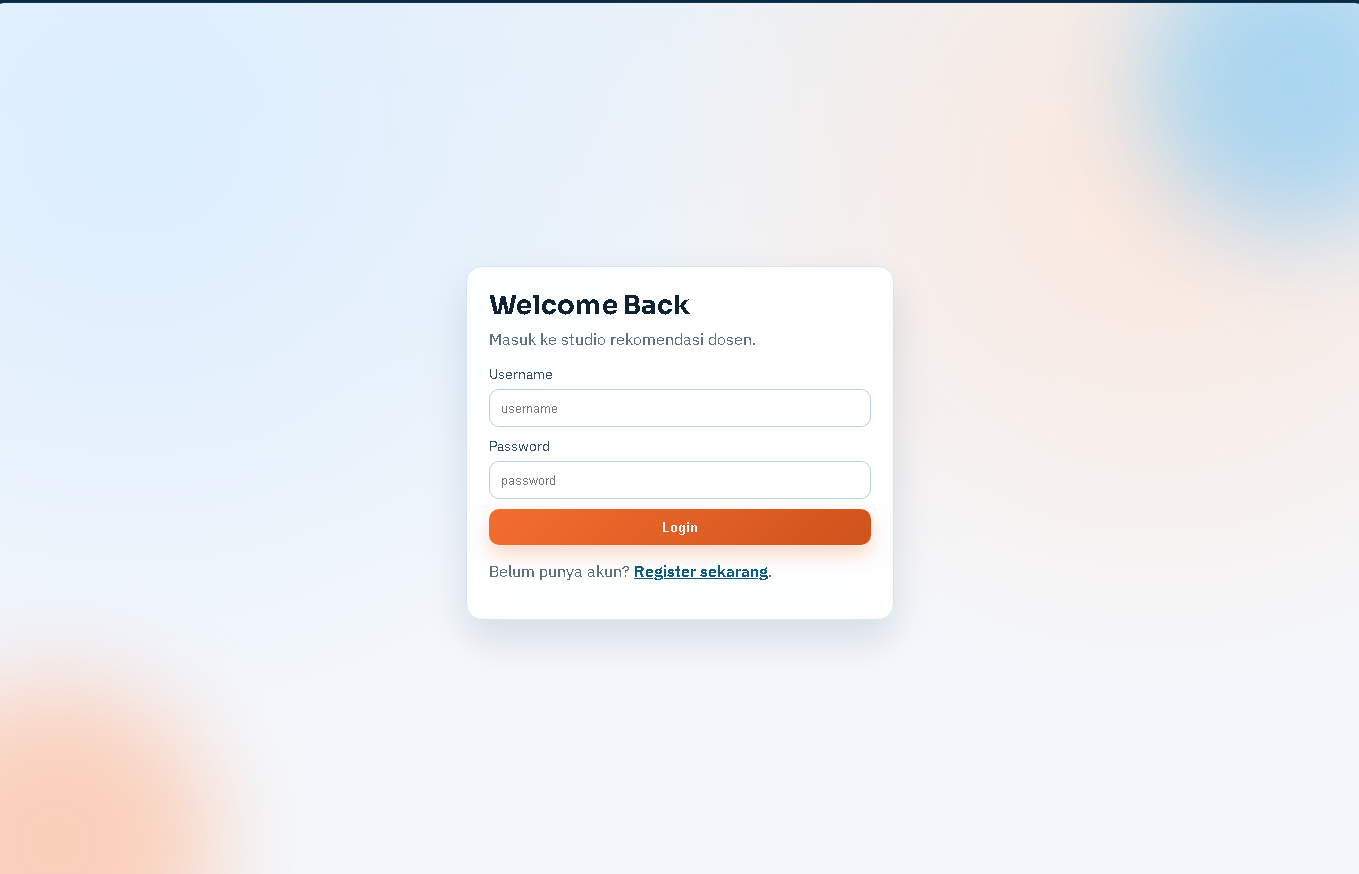
\includegraphics[width=0.7\linewidth]{pic/login.png}
    \end{center}
    \caption{Tampilan Halaman Login}
    \label{fig:login}
\end{figure}
        
Halaman login merupakan gerbang utama interaksi pengguna dengan sistem yang menyediakan formulir terstruktur untuk memasukkan data kredensial. Antarmuka (interface) ini mencakup kolom (field) username dan kata sandi yang telah didaftarkan oleh pengguna sebelumnya. Juga bila pengguna belum memiliki akun bisa mendaftarkan akun dengan memilih tombol registrasi. 

\subsubsection{Register Page}

\begin{figure}
    \begin{center}
        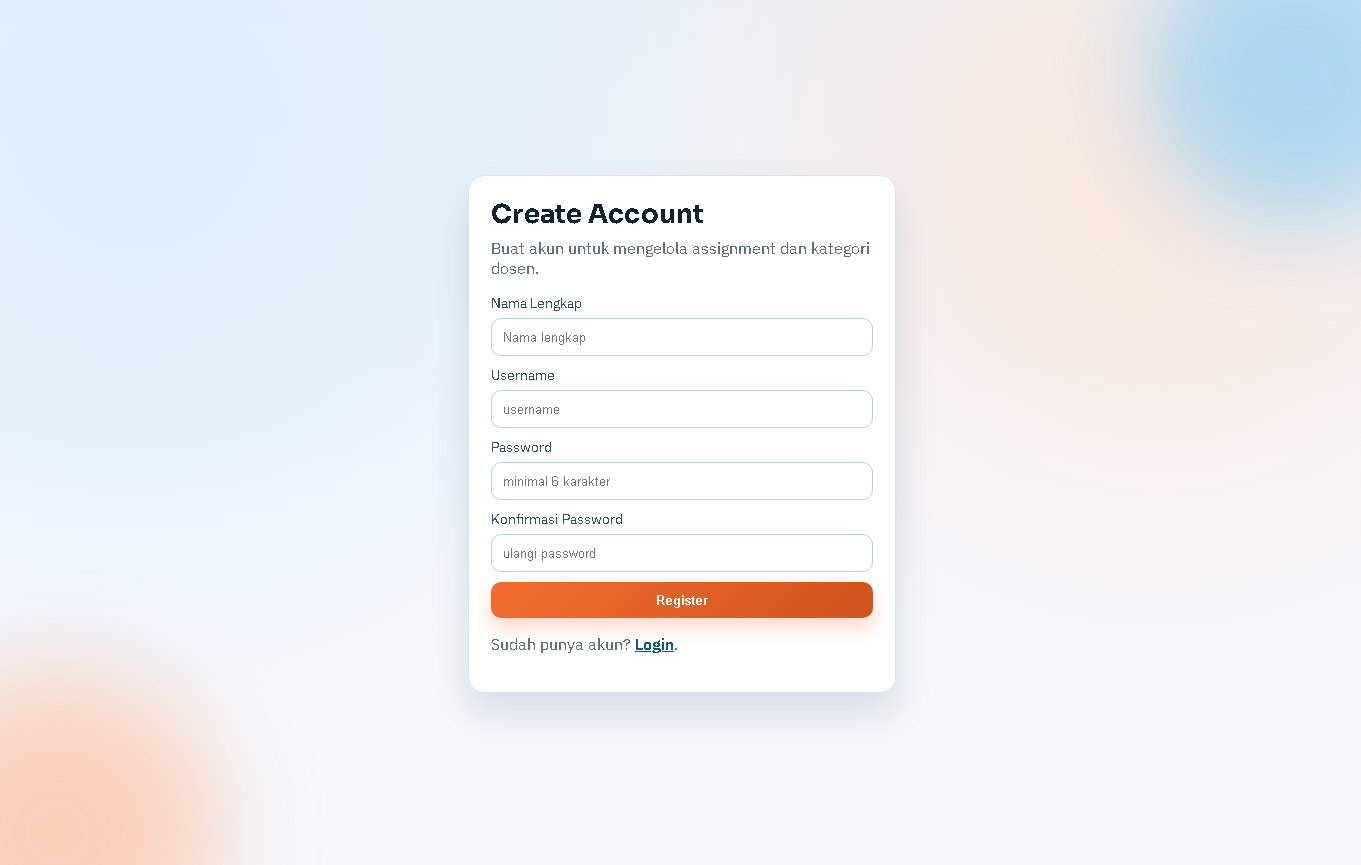
\includegraphics[width=0.7\linewidth]{pic/register.png}
    \end{center}
    \caption{Tampilan Halaman Register}
    \label{fig:register}
\end{figure}
        
Pada halaman ini pengguna dapat membuat akun dengan mengisi beberapa fields seperti nama lengkap, username, password dan konfirmasi password. Lalu proses dilanjutkan dengan memilih tombol registrasi setelah mengisi data dan akun akan otomatis dibuat. 

\subsubsection{Dashboard}

\begin{figure}
    \begin{center}
        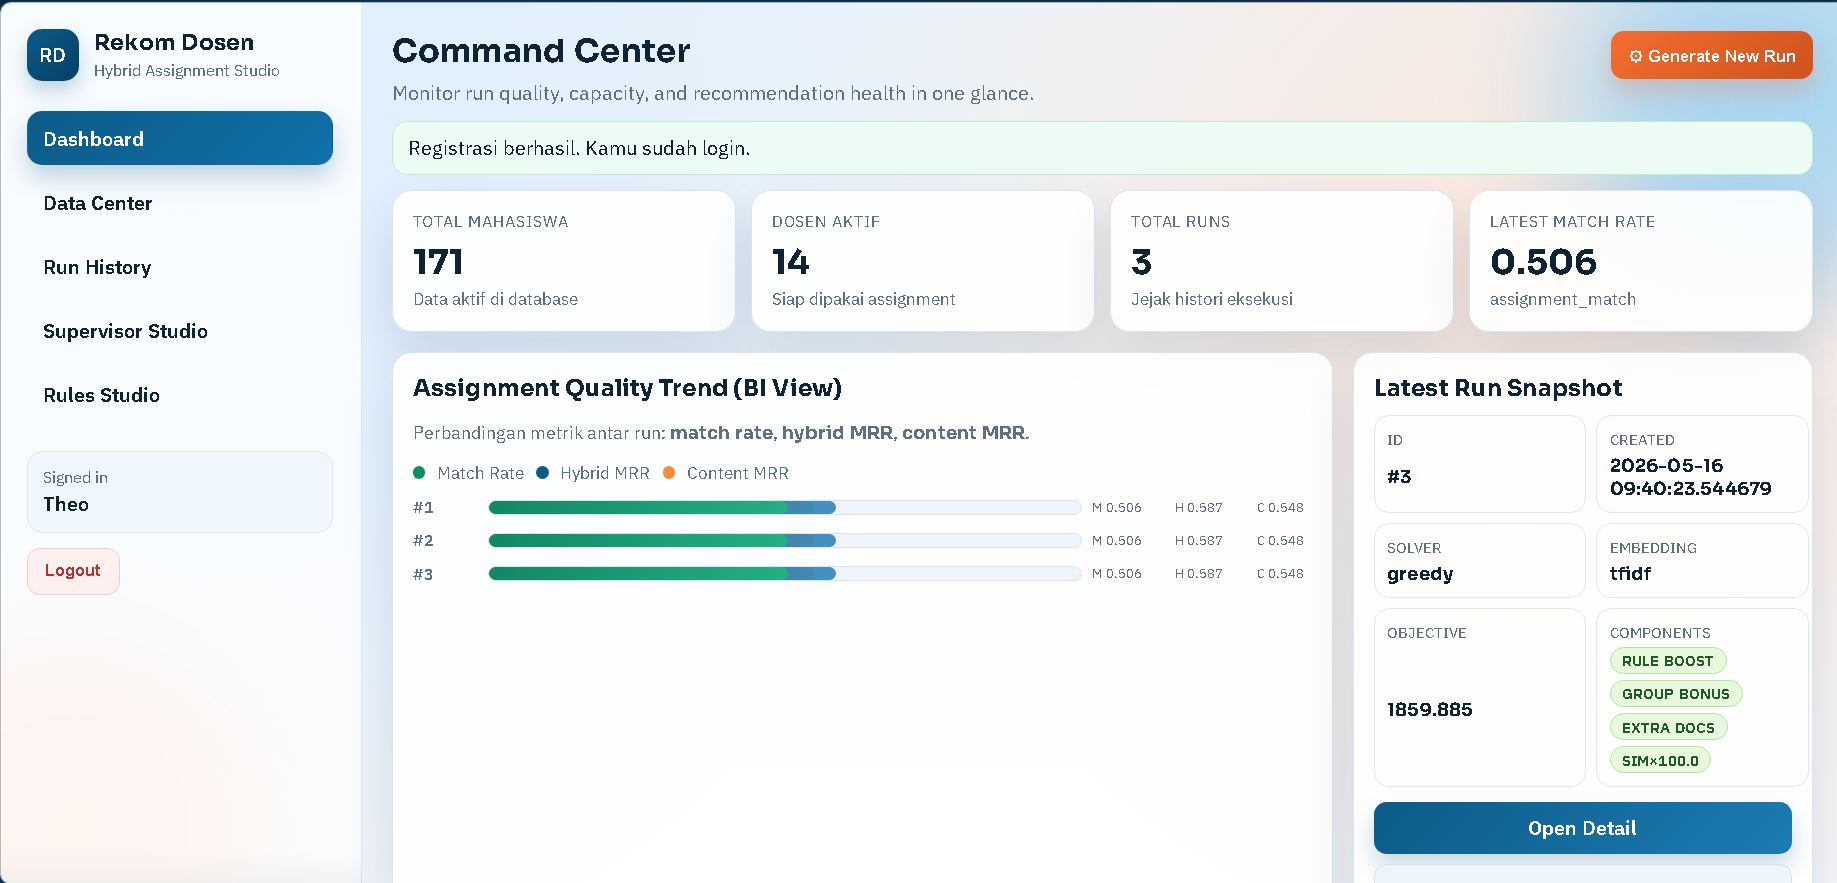
\includegraphics[width=0.7\linewidth]{pic/dashboard.png}
    \end{center}
    \caption{Tampilan Halaman Dashboard}
    \label{fig:dashboard}
\end{figure}
        
Halaman dashboard menyajikan ringkasan data statistik utama, meliputi total mahasiswa dan dosen yang telah terdaftar di dalam sistem. Selain itu, pengguna dapat memantau akumulasi proses eksekusi (total runs), tingkat akurasi pada eksekusi terakhir, serta rincian hasil evaluasi yang telah diproses. Fitur pada halaman ini juga memungkinkan pengguna untuk mengakses rincian run, dan inspect row, hingga melakukan ekspor data ke format Excel berdasarkan hasil eksekusi terbaru.  
\subsubsection{Data Center}

\begin{figure}
    \begin{center}
        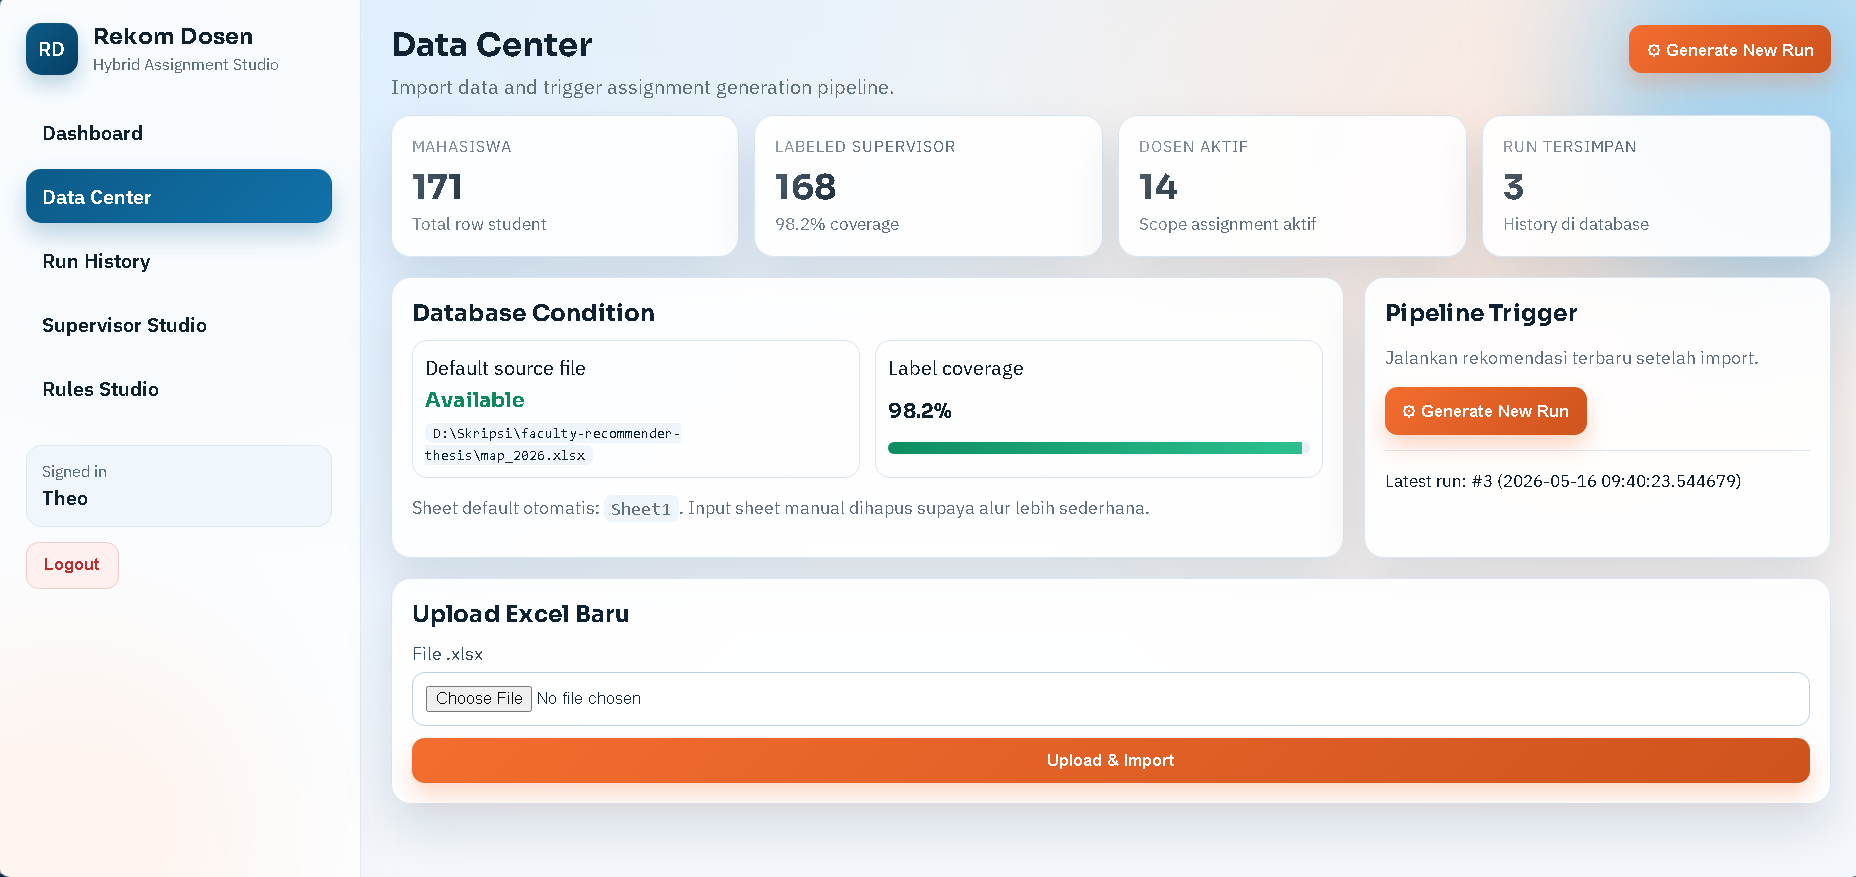
\includegraphics[width=0.7\linewidth]{pic/datacenter.png}
    \end{center}
    \caption{Tampilan Halaman Data Center}
    \label{fig:datacenter}
\end{figure}
        
Halaman ini berfungsi sebagai pusat pengelolaan data masukan (dataset) serta pengendali eksekusi awal (pipeline trigger) sistem. Peran utamanya adalah melakukan proses ETL (Extract, Transform, Load) guna memastikan kesiapan data mahasiswa dan dosen pembimbing sebelum diproses oleh algoritma rekomendasi. 

\subsubsection{Run History}

\begin{figure}
    \begin{center}
        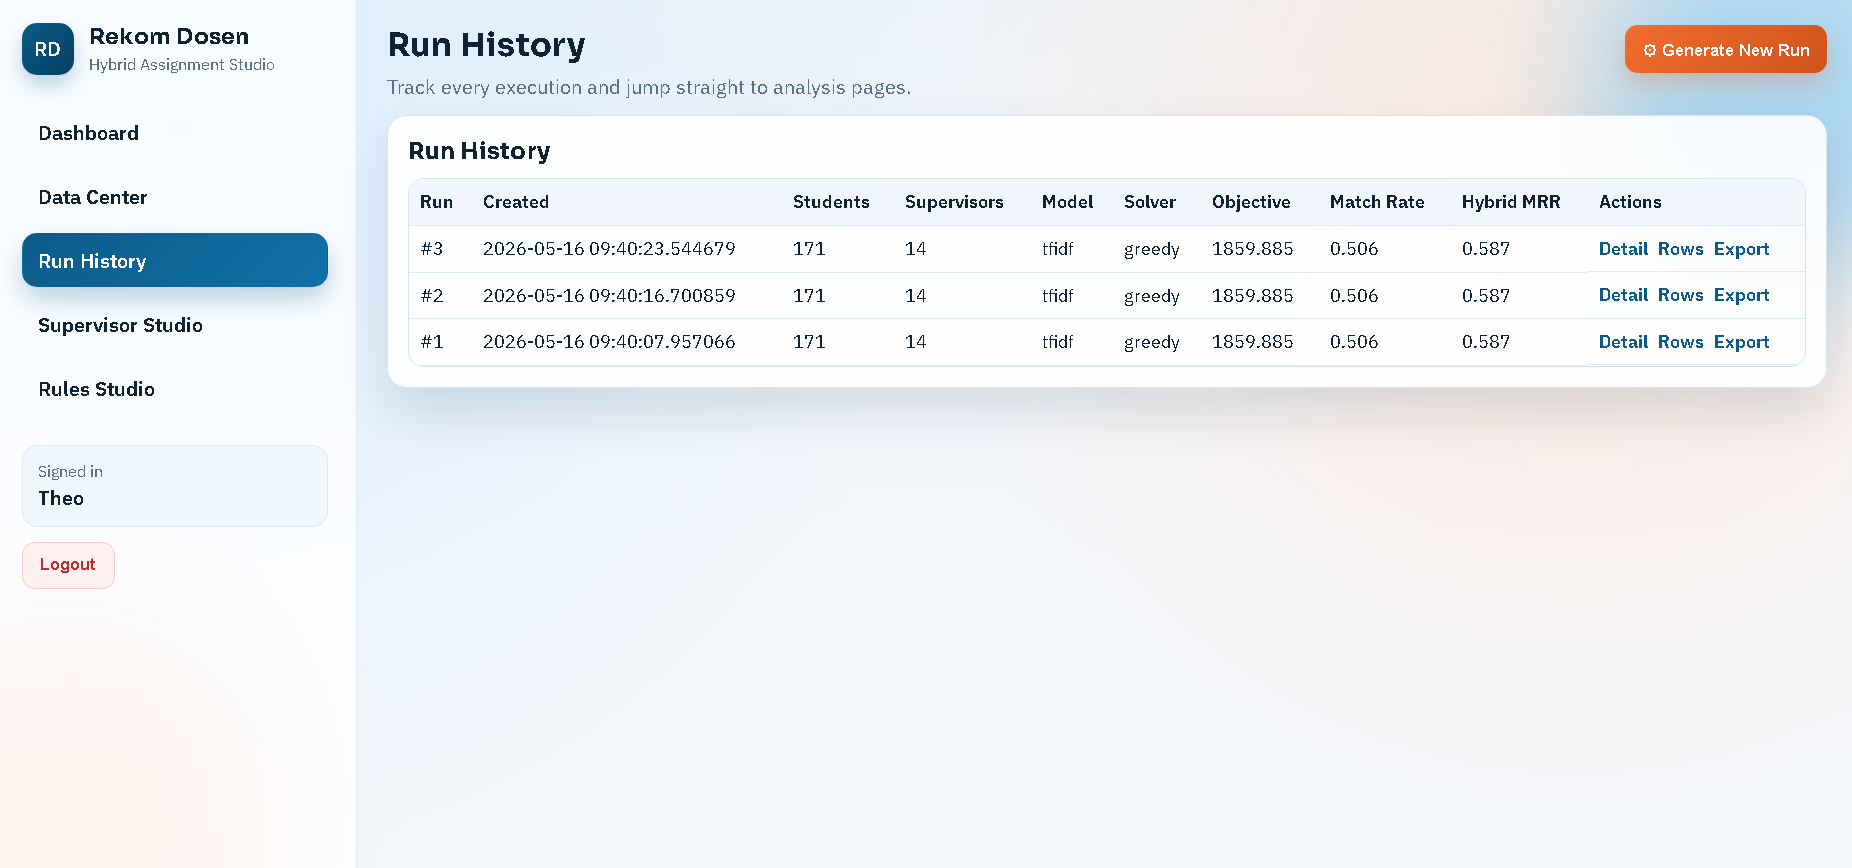
\includegraphics[width=0.7\linewidth]{pic/runhistory.png}
    \end{center}
    \caption{Tampilan Halaman Run History}
    \label{fig:runhistory}
\end{figure}
        
Halaman Run History menyajikan riwayat seluruh proses eksekusi run yang telah dilakukan oleh sistem. Informasi yang ditampilkan mencakup waktu eksekusi, jumlah mahasiswa dan dosen yang terlibat, model yang digunakan, serta hasil evaluasinya. Selain itu, pengguna dapat melakukan aksi lanjutan untuk meninjau rincian eksekusi detail run maupun mengekspor data ke dalam format Excel.   

\subsubsection{Run Details}

\begin{figure}
    \begin{center}
        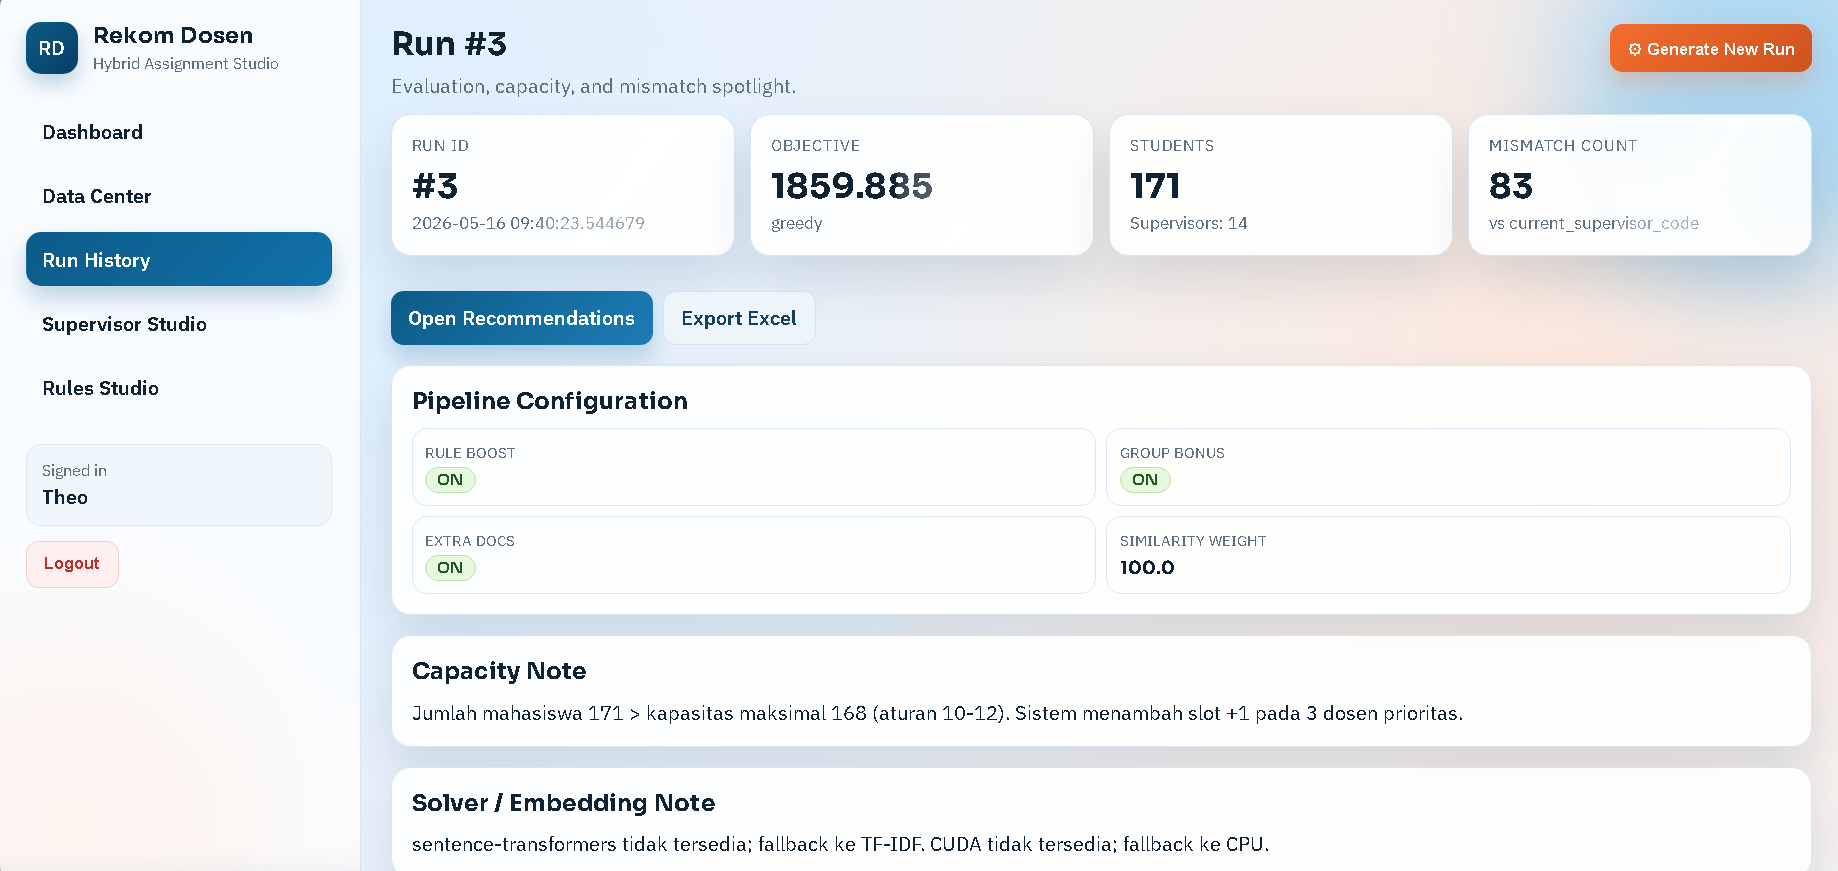
\includegraphics[width=0.7\linewidth]{pic/rundetails.png}
    \end{center}
    \caption{Tampilan Halaman Run Details}
    \label{fig:rundetails}
\end{figure}
        
Halaman Run Details menampilkan rincian hasil dari proses eksekusi run yang telah dilakukan. Informasi yang disajikan mencakup data spesifik untuk setiap mahasiswa, meliputi NIM, Nama, Track, Partner, Topik, Current Supervisor, Recommended Supervisor, Final Score, dan Rule Match. Selain itu, pengguna dapat menggunakan fitur filter untuk mempermudah pencarian data berdasarkan parameter tertentu, seperti nama, topik, maupun dosen  supervisor tertentu. . 

\subsubsection{Supervisor Studio}

\begin{figure}
    \begin{center}
        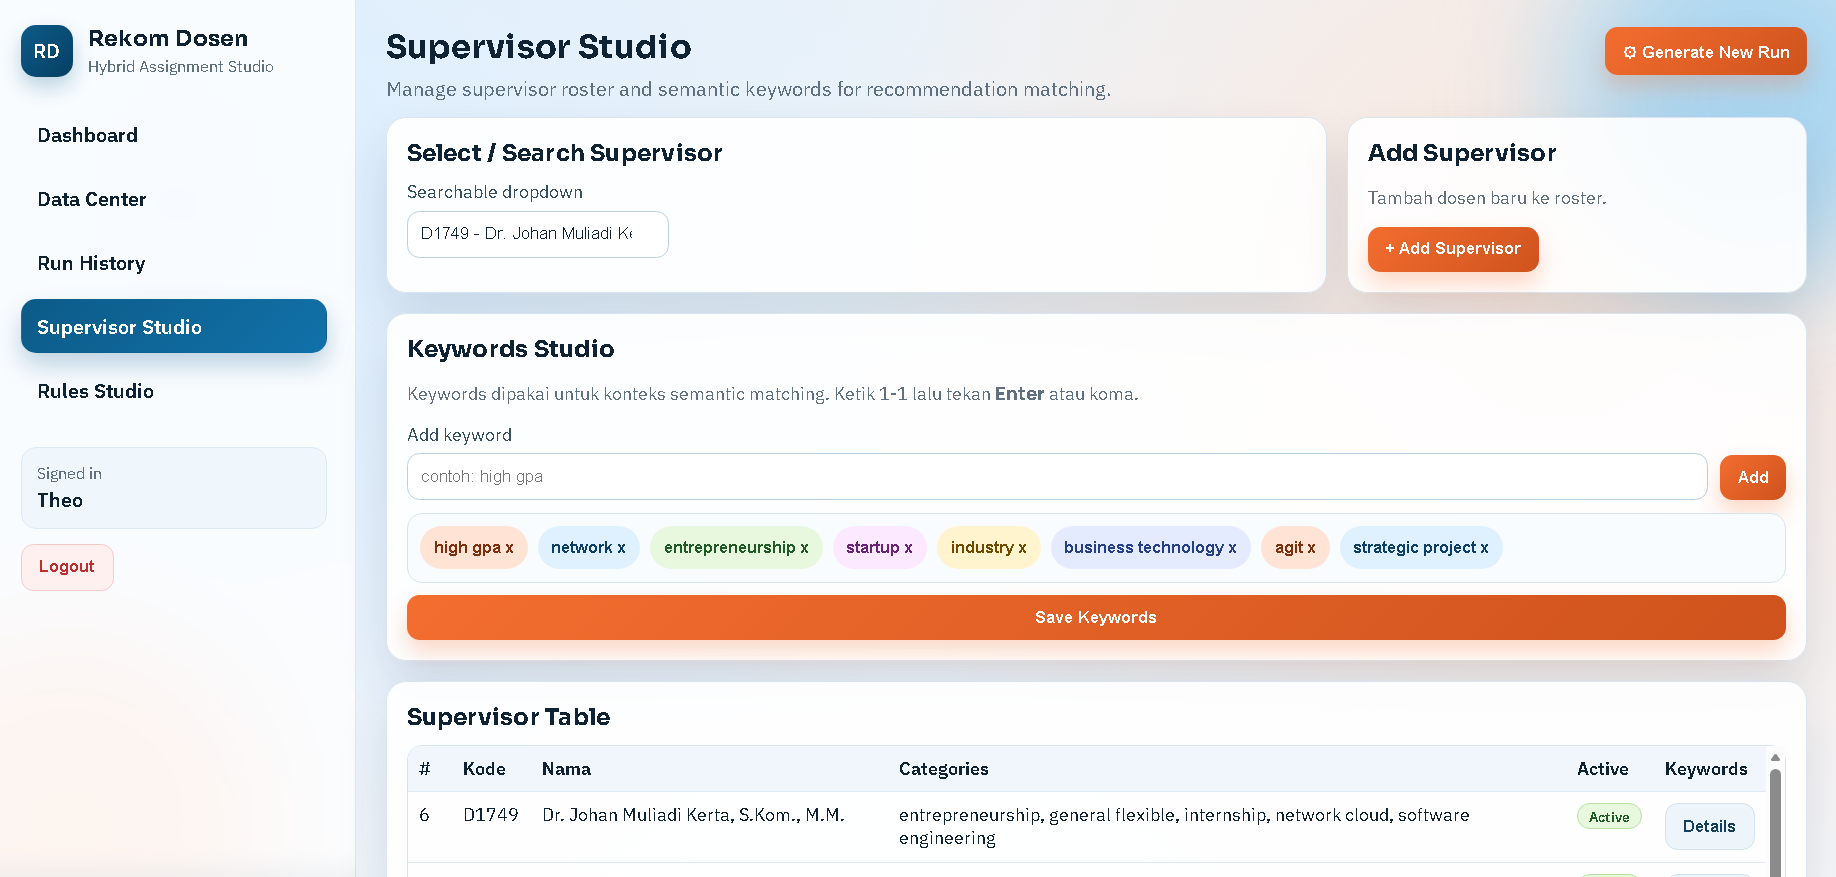
\includegraphics[width=0.7\linewidth]{pic/supervisorstudio.png}
    \end{center}
    \caption{Tampilan Halaman Supervisor Studio}
    \label{fig:supervisorstudio}
\end{figure}
        
Halaman Supervisor Studio berfungsi mengelola repositori dosen pembimbing dan semantic keywords. Fitur utama halaman ini meliputi searchable dropdown dan tombol Load Supervisor untuk pemanggilan profil dosen, serta Export Config Excel untuk pencadangan data. Selain itu, terdapat formulir Add Supervisor untuk perekaman data dosen baru, panel Keywords Studio untuk memanipulasi komponen chip kata kunci secara dinamis, dan Supervisor Table yang menyajikan akumulasi data dosen terdaftar secara terstruktur. 

\subsubsection{Rules Studio}

\begin{figure}
    \begin{center}
        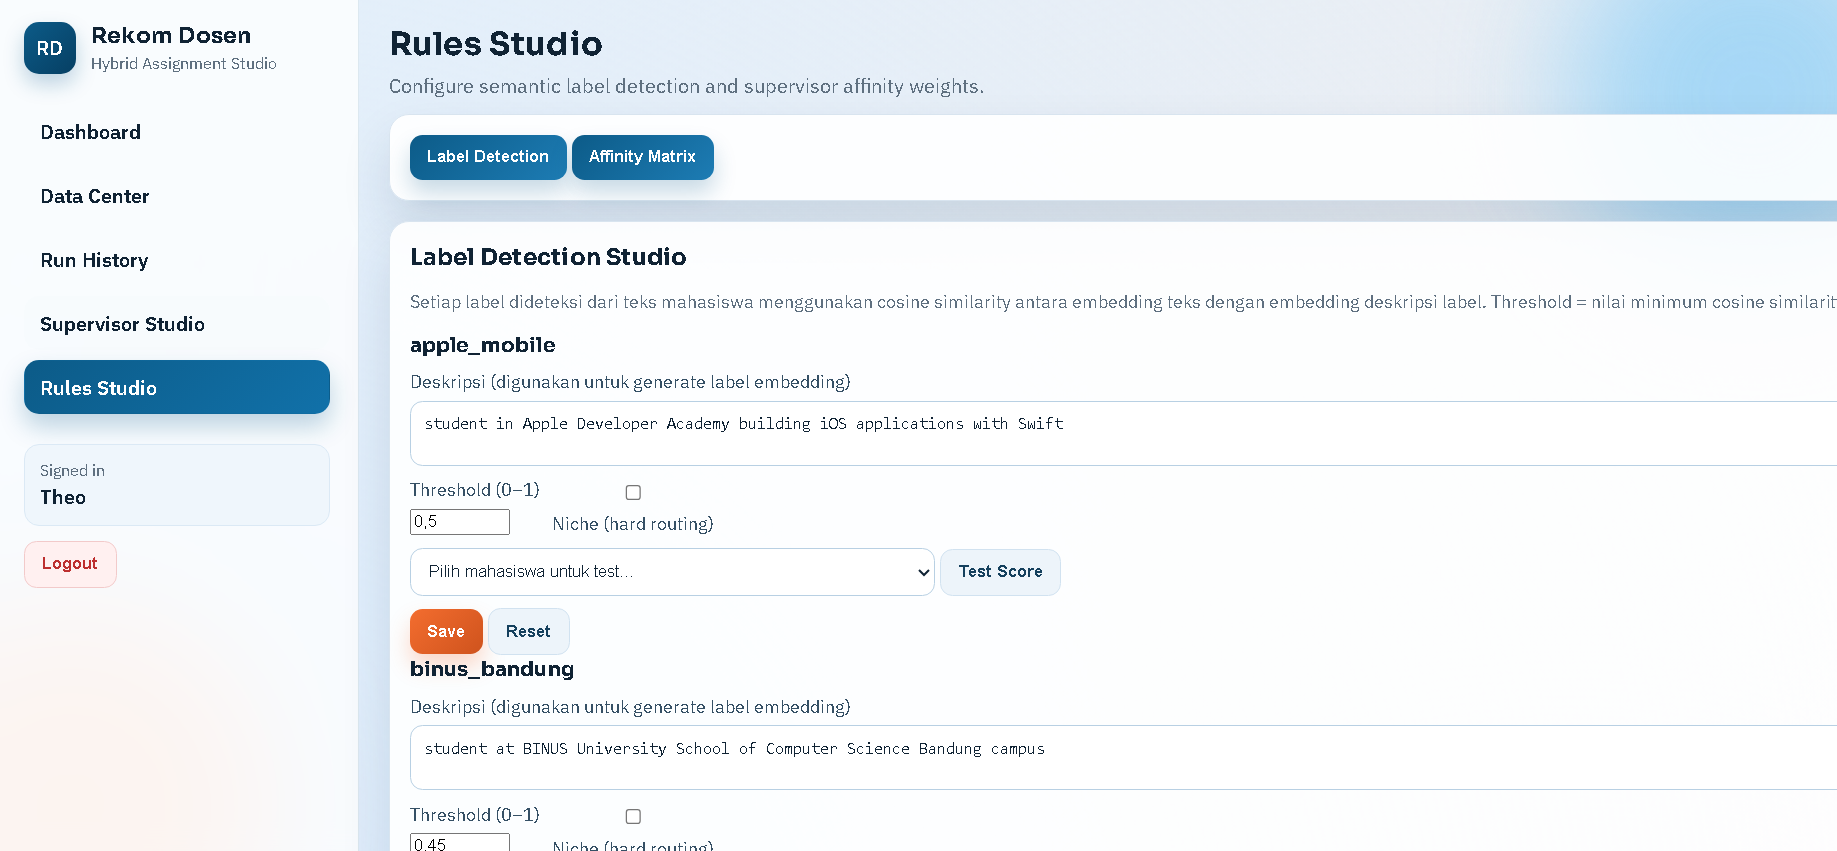
\includegraphics[width=0.7\linewidth]{pic/rulestudio.png}
    \end{center}
    \caption{Tampilan Halaman Rules Studio}
    \label{fig:rulestudio}
\end{figure}

Halaman Rules Studio berfungsi mengonfigurasi parameter klasifikasi label semantik yang digunakan dalam proses rekomendasi. Fitur utama meliputi pengaturan \textit{cosine similarity threshold} per label semantik, pengelolaan deskripsi label yang menentukan pemetaan profil mahasiswa ke kategori penugasan tertentu (seperti \texttt{apple\_mobile} atau \texttt{binus\_bandung}), serta pratinjau skor label untuk profil mahasiswa tertentu. Perubahan konfigurasi pada halaman ini akan berpengaruh pada proses deteksi label pada \textit{pipeline} run berikutnya.

\section{Evaluasi}

Pengujian Black Box dilakukan untuk memvalidasi fungsionalitas sistem dari sudut pandang pengguna tanpa melihat struktur kode internal. Fokus pengujian ini adalah memastikan bahwa setiap input memberikan output yang sesuai dengan spesifikasi kebutuhan sistem. Metode yang digunakan adalah Equivalence Partitioning, di mana data uji dibagi ke dalam beberapa kategori untuk menguji perilaku sistem terhadap input yang valid dan tidak valid. 

\subsection{Login Page}

Pada halaman ini terdapat tombol “Login” yang akan mengarahkan pengguna jika mengisi kredensial dengan benar. 

\begin{table}
 \centering
\begin{tabular}{|>{\fontsize{11}{14}\selectfont}p{0.5cm}|>{\fontsize{11}{14}\selectfont}p{4cm}|>{\fontsize{11}{14}\selectfont}p{3cm}|>{\fontsize{11}{14}\selectfont}p{4cm}|>{\fontsize{11}{14}\selectfont}p{1cm}|}
    \hline
\textbf{No} & \textbf{Skenario Pengujian} & \textbf{Data Uji} & \textbf{Hasil yang Diharapkan} & \textbf{Status }\\
    \hline
    1 & Login dengan kredensial valid  & Email dan kata sandi benar & Sistem mengarahkan pengguna ke dashboard & Pass  \\ 
    \hline
    2 & Login dengan kata sandi salah   & Email benar, kata sandi salah  & Sistem menampilkan message “Kredential Salah” & Pass  \\ 
    \hline
    3 & Login dengan email salah   &Email salah, kata sandi benar  &Sistem menampilkan message “Kredential Salah”  & Pass  \\ 
    \hline
\end{tabular}
\renewcommand{\arraystretch}{1}
	\caption{Skenario Login Page}
	\label{table:tab4.3.1}
\end{table}

\subsection{Register Page}

Pada halaman ini pengguna dapat membuat akun dengan mengisi data email dan password sebagai kredensial.

\begin{table}
 \centering
\begin{tabular}{|>{\fontsize{11}{14}\selectfont}p{0.5cm}|>{\fontsize{11}{14}\selectfont}p{4cm}|>{\fontsize{11}{14}\selectfont}p{3cm}|>{\fontsize{11}{14}\selectfont}p{4cm}|>{\fontsize{11}{14}\selectfont}p{1cm}|}
    \hline
\textbf{No} & \textbf{Skenario Pengujian} & \textbf{Data Uji} & \textbf{Hasil yang Diharapkan} & \textbf{Status }\\
    \hline
    1 & Mendaftarkan akun dengan email dan password   & Email dan kata sandi benar & Sistem menyimpan data email dan password pengguna & Pass  \\ 
    \hline
   2 & Mendaftarkan akun dengan kata sandi salah    & Email benar, kata sandi salah  & Sistem menampilkan message “Data tidak sesuai” & Pass  \\ 
    \hline
    3 & Mendaftarkan akun email salah    &Email salah, kata sandi benar  &Sistem menampilkan message “Data tidak sesuai”  & Pass  \\ 
    \hline
\end{tabular}
\renewcommand{\arraystretch}{1}
	\caption{Skenario Register Page}
	\label{table:tab4.4}
\end{table}

\subsection{Dashboard}

Pada halaman ini bertujuan pada fungsionalitas visual dan interaksi pada halaman Dashboard. Pengujian mencakup validasi tampilan data statistik, grafik tren, detail eksekusi terbaru, dan kontrol navigasi.

\begin{table}
 \centering
\begin{tabular}{|>{\fontsize{11}{14}\selectfont}p{0.5cm}|>{\fontsize{11}{14}\selectfont}p{4cm}|>{\fontsize{11}{14}\selectfont}p{3cm}|>{\fontsize{11}{14}\selectfont}p{4cm}|>{\fontsize{11}{14}\selectfont}p{1cm}|}
    \hline
\textbf{No} & \textbf{Skenario Pengujian} & \textbf{Data Uji} & \textbf{Hasil yang Diharapkan} & \textbf{Status }\\
    \hline
    1 & Klik Menu "Dashboard"   & - & Sistem mengarahkan pengguna ke halaman Data Center  & Pass  \\ 
    \hline
   2 & Klik menu “Run History”  & -  & Sistem mengarahkan pengguna ke halaman Run History  & Pass  \\ 
    \hline
    3 &Klik menu “Supervisor Studio”     & -  & Sistem mengarahkan pengguna ke halaman Supervisor Studio   & Pass  \\ 
    \hline
     4 &Klik menu “Rules Studio”      & -  & Sistem mengarahkan pengguna ke halaman Rules Studio    & Pass  \\ 
    \hline
     5 & Klik tombol “Generate New Run”      & -  & Sistem akan mengarahkan pengguna ke tampilan untuk melakukan run baru    & Pass  \\ 
    \hline
     6 & Klik tombol “Open Detail”      & -  & Sistem mengarahkan pengguna ke halaman detail dari run terakhir   & Pass  \\ 
    \hline
     7 & Klik tombol “Inspect Rows”       & -  & Sistem akan mengarahkan pengguna melihat data pada Run History   & Pass  \\ 
    \hline
     8 & Klik tombol “Export Excel”      & -  & Sistem akan melakukan export pada data run terakhir.    & Pass  \\ 
    \hline
    9 & Sistem menampilkan data pada Summary Cards       & -  & Data yang ditampilkan sesuai dengan database   & Pass  \\ 
    \hline
    10 & Sistem menampikan data pada Quality Trend      & -  & Sistem menampikan tooltop detail nilai Match Rate, Hybrid MRR, dan Content MRR    & Pass  \\ 
    \hline
    11 & Sistem menampikan Informasi Snapshot      & -  & Sistem menampilkan data dari run paling baru     & Pass  \\ 
    \hline
\end{tabular}
\renewcommand{\arraystretch}{1}
	\caption{Skenario Dashboard}
	\label{table:tab4.5}
\end{table}

\subsection{Data Center}

Pada halaman ini pengujian bertujuan untuk memvalidasi fungsi manajemen  import data serta interaksi pipeline trigger. Halaman ini krusial karena bertindak sebagai penyedia data utama sebelum sistem menjalankan algoritma rekomendasi. 

\begin{table}
 \centering
\begin{tabular}{|>{\fontsize{11}{14}\selectfont}p{0.5cm}|>{\fontsize{11}{14}\selectfont}p{4cm}|>{\fontsize{11}{14}\selectfont}p{3cm}|>{\fontsize{11}{14}\selectfont}p{4cm}|>{\fontsize{11}{14}\selectfont}p{1cm}|}
    \hline
\textbf{No} & \textbf{Skenario Pengujian} & \textbf{Data Uji} & \textbf{Hasil yang Diharapkan} & \textbf{Status }\\
    \hline
    1 & Upload Data Kosong   & - & Sistem menolak proses import dan menampikan error message  & Pass  \\ 
    \hline
   2 & Upload Data dengan Format Salah  & -  & Sistem menolak proses import dan menampilkan  error message   & Pass  \\ 
    \hline
    3 & Upload Valid     & -  & File berhasil disimpan, dan sistem akan menampilkan data pada sumarry cards.    & Pass  \\ 
    \hline
     4 & Data pada Summary Cards sesuai      & -  & Data yang ditampilkan sesuai dengan data upload     & Pass  \\ 
    \hline
     5 & Klik tombol “Generate New Run”      & -  & Sistem akan mengarahkan pengguna ke tampilan untuk melakukan run baru    & Pass  \\ 
    \hline
    
\end{tabular}
\renewcommand{\arraystretch}{1}
	\caption{Skenario Data Center}
	\label{table:tab4.6}
\end{table}

\subsection{Generate New Run}

Pada halaman ini pengujian berfungsi untuk melalukan pengecekan ketika pengguna ingin melakukan run baru dengan memilih model dan rules boost yang akan diterapkan pada run tersebut. 

\begin{table}
 \centering
\begin{tabular}{|>{\fontsize{11}{14}\selectfont}p{0.5cm}|>{\fontsize{11}{14}\selectfont}p{4cm}|>{\fontsize{11}{14}\selectfont}p{3cm}|>{\fontsize{11}{14}\selectfont}p{4cm}|>{\fontsize{11}{14}\selectfont}p{1cm}|}
    \hline
\textbf{No} & \textbf{Skenario Pengujian} & \textbf{Data Uji} & \textbf{Hasil yang Diharapkan} & \textbf{Status }\\
    \hline
    1 & Memilih Model   & - & Model yang dipilih akan terlihat dengan ditandai berwarna oren  & Pass  \\ 
    \hline
   2 & Mengaktifkan Group Bonus  & -  & Toggle group bonus yang dipilih akan berubah warna menjadi oren   & Pass  \\
    \hline
    3 & Menonaktifkan Group Bonus     & -  & Toggle group bonus kembali ke kondisi nonaktif  & Pass  \\ 
    \hline
     4 & Cancel Run     & -  & Sistem akan menutup pop-up new run  \\ 
    \hline
     5 & Eksekusi Run Baru     & -  & Sistem akan menjalankan rekomendasi dengan model dan rules yang dipilih    & Pass  \\ 
    \hline
    
\end{tabular}
\renewcommand{\arraystretch}{1}
	\caption{Skenario Generate New Run}
	\label{table:tab4.7}
\end{table}

\subsection{Run History}

Pada halaman ini  bertujuan untuk memastikan sistem mampu menyajikan daftar riwayat  run algoritma secara kronologis dan akurat. Fokus utama meliputi kebenaran metadata yang ditampilkan serta fungsionalitas button. 

\begin{table}
 \centering
\begin{tabular}{|>{\fontsize{11}{14}\selectfont}p{0.5cm}|>{\fontsize{11}{14}\selectfont}p{4cm}|>{\fontsize{11}{14}\selectfont}p{3cm}|>{\fontsize{11}{14}\selectfont}p{4cm}|>{\fontsize{11}{14}\selectfont}p{1cm}|}
    \hline
\textbf{No} & \textbf{Skenario Pengujian} & \textbf{Data Uji} & \textbf{Hasil yang Diharapkan} & \textbf{Status }\\
    \hline
    1 & Sistem menampikan tabel riwayat run yang sudah dijalankan  & - & Sistem menampilkan kolom Run ID, Created, Students, Supervisor, Model, Solver, Objective, Match Rate, dan Hybrid MRR   & Pass  \\ 
    \hline
   2 & Tabel Riwayat di Tampilkan Berdasarkan Urutan Terakhir Dijalankan  & -  & Data ditampilkan secara urut (Descending)    & Pass  \\ 
    \hline
    3 & Klik tombol “Details Row” pada salah satu ID Run      & -  & Sistem berpindah ke halaman detail page dari run yang dipilih     & Pass  \\ 
    \hline
     4 & Klik tombol “Export Data’ pada salah satu ID Run      & -  & Sistem melakukan export data sesuai ID Run yang dipilih    & Pass  \\ 
    \hline
     5 & Klik tombol “ Generate New Run pada page Run History       & -  & Sistem mengarahkan pengguna ke halaman pembuatan run baru     & Pass  \\ 
    \hline
    
\end{tabular}
\renewcommand{\arraystretch}{1}
	\caption{Skenario Run History}
	\label{table:tab4.8}
\end{table}

\subsection{Supervisor Studio}

Pada halaman ini bertujuan untuk memastikan sistem memvalidasi fitur pengelolaan data dosen pembimbing beserta kata kunci semantik.

\begin{table}
 \centering
\begin{tabular}{|>{\fontsize{11}{14}\selectfont}p{0.5cm}|>{\fontsize{11}{14}\selectfont}p{4cm}|>{\fontsize{11}{14}\selectfont}p{3cm}|>{\fontsize{11}{14}\selectfont}p{4cm}|>{\fontsize{11}{14}\selectfont}p{1cm}|}
    \hline
\textbf{No} & \textbf{Skenario Pengujian} & \textbf{Data Uji} & \textbf{Hasil yang Diharapkan} & \textbf{Status }\\
    \hline
    1 & Membuka menu dropdown dan mencari berdasarkan nama atau kode dosen   & - & Sistem menyaring data secara dinamis berdasarkan data dosen yang dicari    & Pass  \\ 
    \hline
   2 & Memilih salah satu nama dosen kemudian menekan tombol “Load Supervisor”   & -  & Sistem menampilkan profil dosen dan keyword yang sesuai dengan dosen tersebut     & Pass  \\ 
    \hline
    3 & Menekan tombol “Export Config”       & -  & Sistem akan mengunduh berkas excel berisikan data dosen dan profilnya.      & Pass  \\ 
    \hline
     4 & Mengetikkan keyword baru pada kolom “Add Keyword”    & -  & Keyword di daftarkan di dalam daftar keyword     & Pass  \\ 
    \hline
     5 & Menekan tombol (X) pada salah satu komponen chip       & -  & Chip keyword akan dihapuskan       & Pass  \\ 
    \hline
     6 & Menekan tombol “Save Keywords” setelah melakukan perubahan chip       & -  & Sistem memperbarui daftar keyword semantik pada dosen di database        & Pass  \\ 
    \hline
    
\end{tabular}
\renewcommand{\arraystretch}{1}
	\caption{Skenario Supervisor Studio}
	\label{table:tab4.9}
\end{table}


\subsection{Rules Studio}

Pada halaman ini testing bertujuan untuk memvalidasi fleksibilitas pengaturan rules. Halaman ini mengontrol cosine similarity threshold dan deskripsi label semantik yang menentukan bagaimana profil minat mahasiswa dipetakan ke dalam kategori penugasan tertentu (seperti apple\_mobile atau binus\_bandung).  

\begin{table}
 \centering
\begin{tabular}{|>{\fontsize{11}{14}\selectfont}p{0.5cm}|>{\fontsize{11}{14}\selectfont}p{4cm}|>{\fontsize{11}{14}\selectfont}p{3cm}|>{\fontsize{11}{14}\selectfont}p{4cm}|>{\fontsize{11}{14}\selectfont}p{1cm}|}
    \hline
\textbf{No} & \textbf{Skenario Pengujian} & \textbf{Data Uji} & \textbf{Hasil yang Diharapkan} & \textbf{Status }\\
    \hline
    1 & Membuka menu dropdown dan mencari berdasarkan nama atau kode dosen   & - & Sistem menyaring data secara dinamis berdasarkan data dosen yang dicari    & Pass  \\ 
    \hline
   2 & Memilih salah satu nama dosen kemudian menekan tombol “Load Supervisor”   & -  & Sistem menampilkan profil dosen dan keyword yang sesuai dengan dosen tersebut     & Pass  \\ 
    \hline
    3 & Menekan tombol “Export Config”       & -  & Sistem akan mengunduh berkas excel berisikan data dosen dan profilnya.      & Pass  \\ 
    \hline
     4 & Mengetikkan keyword baru pada kolom “Add Keyword”    & -  & Keyword di daftarkan di dalam daftar keyword     & Pass  \\ 
    \hline
     5 & Menekan tombol (X) pada salah satu komponen chip       & -  & Chip keyword akan dihapuskan       & Pass  \\ 
    \hline
     6 & Menekan tombol “Save Keywords” setelah melakukan perubahan chip       & -  & Sistem memperbarui daftar keyword semantik pada dosen di database        & Pass  \\ 
    \hline
    
\end{tabular}
\renewcommand{\arraystretch}{1}
	\caption{Skenario Supervisor Studio}
	\label{table:tab4.10}
\end{table}

% % Bab 5 : Kesimpulan dan Saran
%---------------------------------------------------------------
\chapter{\babLima}
%\begin{center}
%	\textbf{BAB IV}
%	\par \textbf{ANALISIS SIMULASI SISTEM}
%\end{center}

\section{Simpulan}

Penelitian ini bertujuan untuk mengembangkan sistem rekomendasi \textit{Faculty Supervisor} berbasis \textit{semantic similarity} sebagai pendukung keputusan dalam proses pemetaan mahasiswa peserta Program Enrichment di XYZ University. Berdasarkan hasil analisis, perancangan, implementasi, dan evaluasi yang telah dilakukan, dapat ditarik simpulan yang disusun untuk menjawab ketiga rumusan masalah penelitian sebagai berikut.

\begin{enumerate}
    \item Menjawab rumusan masalah pertama, sistem rekomendasi \textit{Faculty Supervisor} magang berbasis website telah berhasil dirancang dan dikembangkan menggunakan pendekatan \textit{semantic similarity} dengan arsitektur \textit{Transformer} (model BAAI/bge-m3). Sistem ini menggabungkan skor kemiripan semantik, aturan \textit{company group bonus}, dan algoritma \textit{greedy capacity solver} untuk menjaga keseimbangan kuota pembimbingan setiap dosen.

    \item Menjawab rumusan masalah kedua, tingkat kesesuaian hasil rekomendasi sistem dengan \textit{ground truth} penugasan institusional tergolong tinggi. Pengujian menghasilkan \textit{Mean Reciprocal Rank} (MRR) sebesar 0,711, Hit@5 sebesar 0,929, dan \textit{Assignment Match Rate} sebesar 0,530, yang menunjukkan bahwa pembimbing relevan secara konsisten muncul pada peringkat teratas rekomendasi.

    \item Menjawab rumusan masalah ketiga, sistem yang dikembangkan terbukti meningkatkan efisiensi proses pemetaan \textit{Faculty Supervisor} magang oleh EPC. Waktu penentuan yang sebelumnya membutuhkan 1 hingga 3 minggu per \textit{batch} dapat dipersingkat menjadi hitungan menit, dengan proses yang lebih terotomatisasi, transparan, dan objektif, serta sebaran beban pembimbingan yang sangat merata antar dosen, ditandai dengan nilai \textit{Gini Coefficient} sebesar 0,0138.

\end{enumerate}

\section{Saran}

Berdasarkan hasil penelitian yang telah dilakukan, terdapat beberapa saran untuk pengembangan lebih lanjut:

\begin{enumerate}
    \item \textbf{Perluasan cakupan data supervisor.} Representasi dosen pembimbing saat ini bergantung pada data historis bimbingan dan rekomendasi topik skripsi yang tersedia. Penambahan sumber data seperti publikasi ilmiah, profil penelitian, atau portofolio proyek dosen dapat memperkaya representasi semantik dan meningkatkan kualitas rekomendasi.

    \item \textbf{Perluasan cakupan program enrichment.} Sistem yang dikembangkan saat ini difokuskan pada jalur magang (\textit{internship}). Pengembangan selanjutnya dapat mencakup jalur lain dalam Program Enrichment, seperti penelitian (\textit{research}), kewirausahaan (\textit{entrepreneurship}), dan pengembangan profesional, dengan penyesuaian pada skema representasi data mahasiswa.

    \item \textbf{\textit{Fine-tuning} model \textit{embedding} pada domain akademik Indonesia.} Model \textit{embedding} yang digunakan merupakan model \textit{pre-trained} bersifat umum. Melakukan \textit{fine-tuning} pada korpus akademik berbahasa Indonesia atau data spesifik domain Program Enrichment berpotensi meningkatkan akurasi pencocokan semantik secara signifikan.

    \item \textbf{Evaluasi usabilitas dengan pengguna nyata.} Pengujian yang dilakukan dalam penelitian ini terbatas pada \textit{black box testing} fungsional. Evaluasi lanjutan menggunakan \textit{System Usability Scale} (SUS) dengan melibatkan EPC sebagai pengguna nyata perlu dilakukan untuk mengukur tingkat penerimaan dan kemudahan penggunaan sistem secara empiris.

    \item \textbf{Integrasi dengan sistem informasi akademik institusi.} Saat ini sistem memerlukan unggah data manual dalam format Excel. Integrasi langsung dengan sistem informasi akademik XYZ University akan mengurangi potensi kesalahan \textit{input} data dan mempersingkat alur kerja EPC secara keseluruhan.

    \item \textbf{Studi longitudinal terhadap kualitas rekomendasi.} Evaluasi dalam penelitian ini menggunakan data historis satu tahun sebagai \textit{ground truth}. Studi lanjutan yang mengikuti keluaran rekomendasi selama beberapa periode pemetaan akan memberikan gambaran yang lebih representatif terhadap kualitas sistem dalam kondisi operasional nyata.

    \item \textbf{Replikasi sistem ke fakultas lain sebagai uji generalisabilitas.} Evaluasi penelitian ini terbatas pada 168 mahasiswa dan 14 supervisor dari satu program studi dalam satu batch pemetaan. Mengaplikasikan sistem pada fakultas lain dengan skala, komposisi supervisor, dan karakteristik data yang berbeda akan mengonfirmasi apakah model \textit{embedding} dan \textit{greedy solver} yang dikembangkan berperilaku konsisten di luar konteks Computer Science Program Enrichment.
\end{enumerate}



%
% Daftar Pustaka
\renewcommand\bibname{DAFTAR PUSTAKA}
\bibliographystyle{apacite}
\bibliography{ref}
%\includepdf[page=-,pagecommand={},width=\textwidth]{loogbook4}

% Dari sini
% % Lampiran 
% \begin{appendix}
% 	\pagenumbering{gobble}
% 	%
% 
% Hanya sebuah pembatas bertuliskan LAMPIRAN ditengah halaman. 
% 

\begin{titlepage}
	\centering 
	\vspace*{6cm}
	\noindent \Huge{LAMPIRAN}
	\addChapter{LAMPIRAN}
\end{titlepage}


% 	\setcounter{page}{2}
% \end{appendix}

\addChapter{LAMPIRAN}
\addcontentsline{toc}{section}{Lampiran A: Jadwal Kegiatan dan Penelitian}
\addcontentsline{toc}{section}{Lampiran B: Tautan Repository dan Dokumen Pendukung}
\begin{center}
    \Large\bfseries LAMPIRAN
\end{center}
\vspace{1cm}

% === LAMPIRAN 1 ===
\begin{center}
    % Menampilkan gambar surat terlebih dahulu
    % Tinggi disetel 0.73\textheight agar ruang halaman cukup untuk judul LAMPIRAN di atas dan label di bawah
    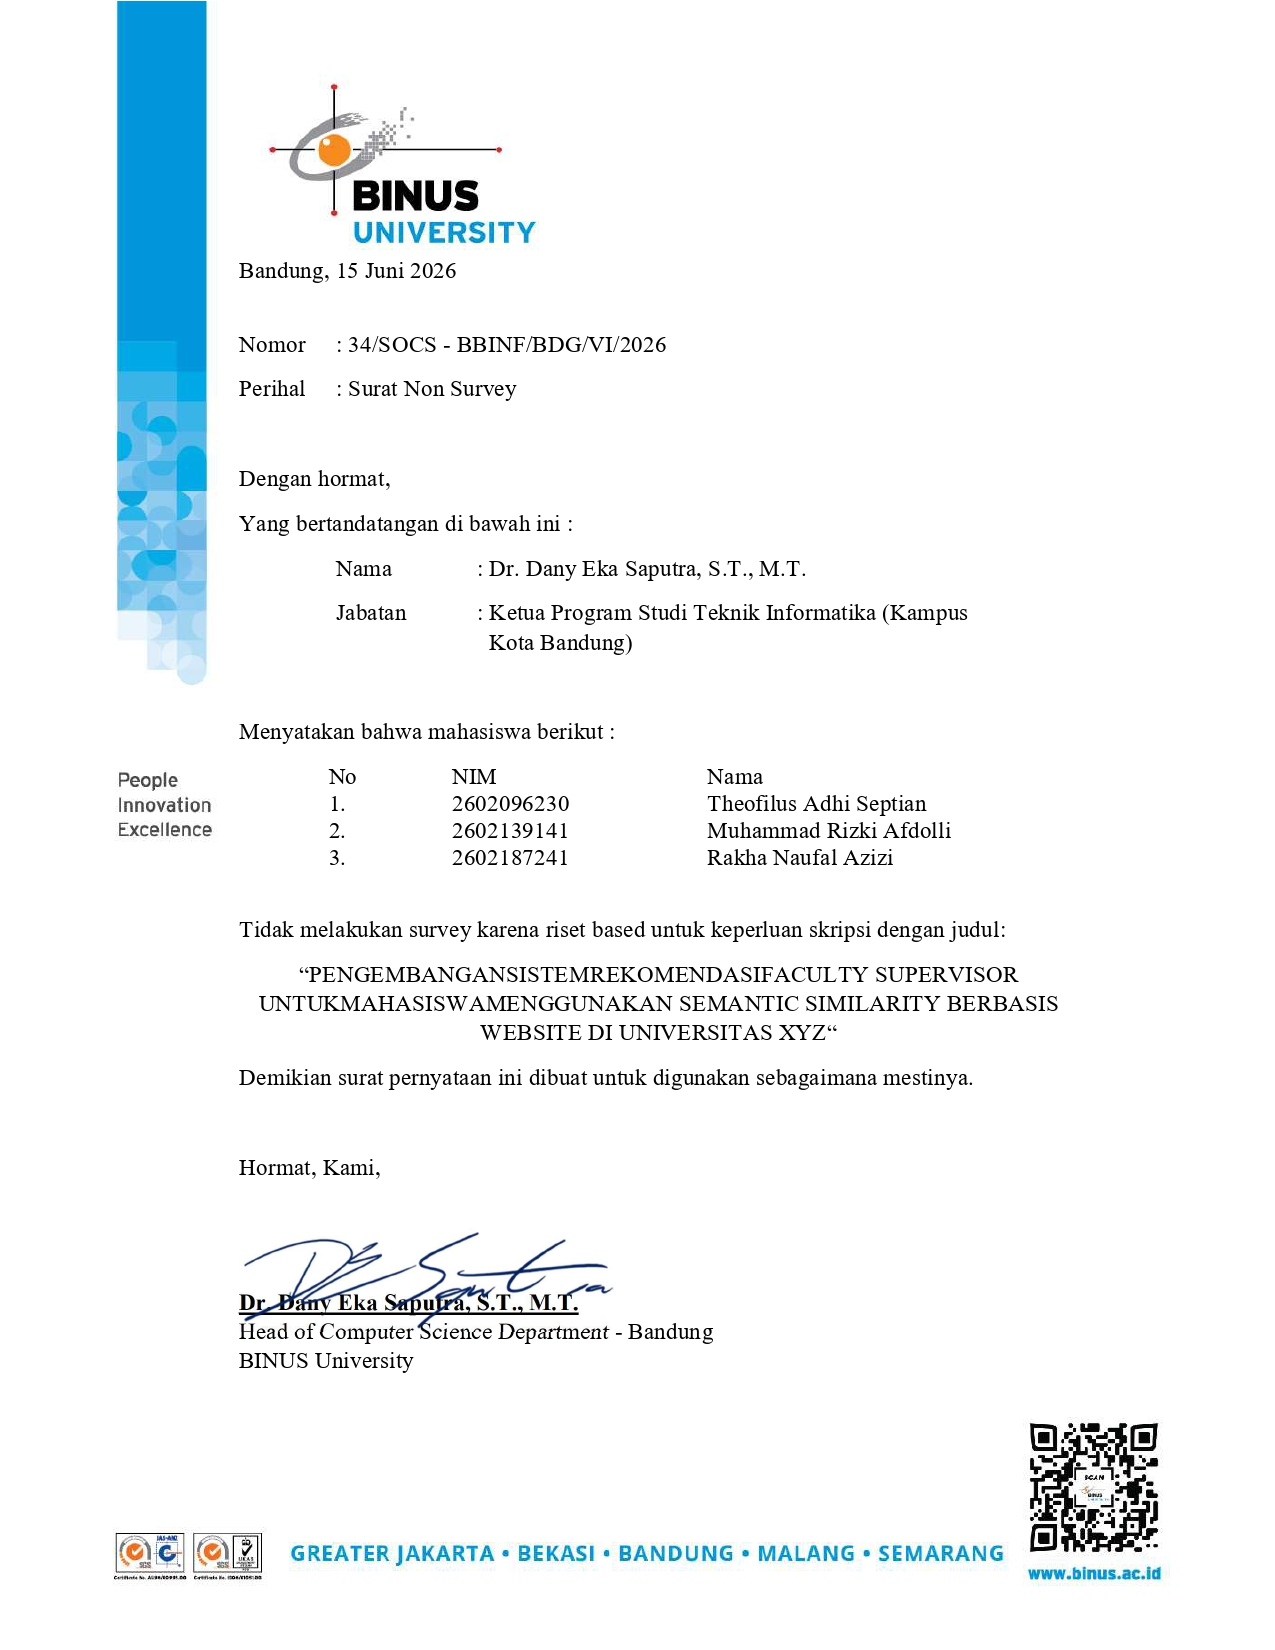
\includegraphics[height=0.73\textheight]{pic/suratsurvey.jpg}
    
    \vspace{0.5cm}
    % Keterangan ditaruh di bawah gambar dengan format miring (italic) sesuai referensi
    \textit{\large Lampiran 1 Surat Survei Mahasiswa}
\end{center}
\newpage

% === LAMPIRAN 2 ===
\noindent\textbf{\large Lampiran 2: Jadwal Kegiatan dan Penelitian}
\vspace{0.4cm}

Berikut adalah jadwal kegiatan penelitian yang dilakukan selama proses pengerjaan skripsi ini, mulai dari bulan September 2025 hingga Juni 2026. [cite: 13, 56, 1653]

\begin{table}[htbp]
\centering
\renewcommand{\thetable}{2.1} % Penomoran otomatis menjadi Tabel 2.1 mengikuti Lampiran 2
\caption{Jadwal Kegiatan Penelitian}
\label{tab:jadwal_kegiatan}
\vspace{0.3cm}

\small 
\setlength{\tabcolsep}{4pt} 

\begin{tabular}{|p{4.8cm}|c|c|c|c|c|c|c|c|c|c|}
\hline
\textbf{Jenis Kegiatan} & \multicolumn{4}{c|}{\textbf{2025}} & \multicolumn{6}{c|}{\textbf{2026}} \\ \cline{2-11} 
 & \textbf{Sep} & \textbf{Okt} & \textbf{Nov} & \textbf{Des} & \textbf{Jan} & \textbf{Feb} & \textbf{Mar} & \textbf{Apr} & \textbf{Mei} & \textbf{Jun} \\ \hline

Studi Literatur dan Tinjauan Pustaka & $\bullet$ & $\bullet$ & & & & & & & & \\ \hline
Analisis Masalah dan Kebutuhan Sistem & & $\bullet$ & $\bullet$ & & & & & & & \\ \hline
Pengumpulan Data Wawancara & & $\bullet$ & & & & & & & & \\ \hline
Penyusunan Bab 1 (Pendahuluan) & & & $\bullet$ & & & & & & & \\ \hline
Penyusunan Bab 2 (Tinjauan Pustaka) & & & $\bullet$ & $\bullet$ & & & & & & \\ \hline
Perancangan Sistem (UML, Arsitektur) & & & $\bullet$ & $\bullet$ & & & & & & \\ \hline
Penyusunan Bab 3 (Metode Penelitian) & & & $\bullet$ & $\bullet$ & & & & & & \\ \hline
Pengembangan Sistem (Implementasi) & & & $\bullet$ & $\bullet$ & $\bullet$ & $\bullet$ & $\bullet$ & $\bullet$ & $\bullet$ & \\ \hline
Pengujian dan Evaluasi Sistem & & & & & & & & $\bullet$ & $\bullet$ & \\ \hline
Penyusunan Bab 4 (Hasil dan Pembahasan) & & & & & & & & $\bullet$ & $\bullet$ & $\bullet$ \\ \hline
Penyusunan Bab 5 (Simpulan dan Saran) & & & & & & & & & $\bullet$ & $\bullet$ \\ \hline
Revisi dan Finalisasi Dokumen & & & & & & & & & & $\bullet$ \\ \hline

\end{tabular}
\end{table}

\newpage

% === LAMPIRAN 3 ===
\noindent\textbf{\large Lampiran 3: Tautan Repository dan Dokumen Pendukung}
\vspace{0.4cm}

Berikut adalah tautan-tautan yang berkaitan dengan penelitian ini, meliputi repositori kode sumber, dokumen skripsi, serta instrumen pengumpulan data. [cite: 1657]
\vspace{0.3cm}

\begin{table}[htbp]
\centering
\renewcommand{\thetable}{3.1} % Penomoran otomatis menjadi Tabel 3.1 mengikuti Lampiran 3
\caption{Daftar Tautan Pendukung Penelitian}
\label{tab:tautan_pendukung}
\vspace{0.3cm}

\small
\begin{tabular}{|c|p{4.5cm}|p{8.5cm}|}
\hline
\textbf{No.} & \textbf{Keterangan} & \textbf{Tautan} \\ \hline

1 & Repository Kode Sumber Sistem Rekomendasi & 
\raggedright \texttt{https://github.com/\allowbreak rizkiafdl/\allowbreak faculty-recommender-thesis} \tabularnewline \hline

2 & Repository Dokumen Skripsi (LaTeX) & 
\raggedright \texttt{https://github.com/\allowbreak rizkiafdl/\allowbreak latex-recomendation-system} \tabularnewline \hline

3 & Google Form Wawancara & 
\raggedright \texttt{https://docs.google.com/\allowbreak forms/d/e/\allowbreak 1FAIpQLSfWDj3e4Xc\allowbreak 2C01WKA1sZ678JEMajcQ\allowbreak 6110aUIOmKWGRgJYQ/\allowbreak viewform?usp=dialog} \tabularnewline \hline

4 & Spreadsheet Hasil Wawancara & 
\raggedright \texttt{https://docs.google.com/\allowbreak spreadsheets/d/\allowbreak 12wOS4fbvfyNWXB5pDLm-\allowbreak ZomiBE5gsTlkulVt\allowbreak U1cvs/edit?usp=sharing} \tabularnewline \hline

\end{tabular}
\end{table}
% Sampe sini buat lampiran

\end{document}